\chapter{FASER: Looking forward for Long-Lived-Particles}
	The Standard Model has proven to be one of the most successful theories in Physics but still fails to address several key phenomena, including the nature itself of DM. This fondamental shortcoming have motivated physicists to explore theoretical extensions of the SM predicting new particles and providing potential DM candidates, many of which remain hidden from current collider experiments due to the their predicted masses but also their often weak coupling to the SM. 

	In the past decades, searches for Beyond the Standard Model (BSM) physics at the LHC was focused on heavy particles in the TeV-scale mass range and couplings to the SM of the order of $\mathcal{O}(1)$. These particles were expected to be produced with large transverse momentum ($p_T$), making large cylindrically symmetric general purpose experiments like ATLAS \cite{atlas_detector} and CMS \cite{cms_detector} the best candidates for detection BSM candidates. 
	
	After many years of searches in this direction, the absence of discoveries opened the floor to an increasingly compelling class of BSM models predicting new particles both light and weakly coupled to the SM \cite{FASER_LLP}, providing good DM candidates. An important aspect of such models is found in the predicted $p_T$ of the particles with masses in the range of MeV-scale to GeV-scale, which can be of the order of $p_T ~ 100$ MeV - GeV and is considerably smaller than the $p_T$ for models predicting particles whose mass belong to the TeV-scale. These particles would hence be produced in what is called the very forward region, making actual searches with experiments like ATLAS completely misguided due to its pseudorapidity coverage roughly limited to $|\eta| \lesssim 2.5$.
	
	This new class of BSM particles often arise in well-motivated models such as hidden sectors connected to the SM via portals—e.g., dark photons (vector portal), axion-like particles (ALPs, pseudoscalar portal) which will be discussed more in details in \note{insert section}, or dark Higgs bosons (scalar portal). At first glance, the extremely weak couplings of these particles to the SM may seem like a showstopper, unless the rate of events from which these particles are originating was sufficiently high. Taking as a benchmark the LHC at $\sqrt{s} =$ \SI{13}{\tera\electronvolt}, the total inelastic proton-proton cross section is approximately $\sigma_{inel}($\SI{13}{\tera\electronvolt}$) \approx 75 \text{ mb}$ \cite{inelastic_XS_ATLAS} of which most it is in the forward direction. The cross section is very similar for the LHC at $\sqrt{s} =$ \SI{14}{\tera\electronvolt} and for an integrated luminosity of 150 fb$^{-1}$, the expected number of inelastic proton-proton scattering is expected to be
	\begin{equation}
		N_{inelastic} \approx 1.1 \cdot 10^{16}
	\end{equation} 

	resulting in extraordinary meson production rates as for example $N_{\pi^0} \approx 2.3 \cdot 10^{17}$ and $N_{B} \approx 7.1 \cdot 10^{13}$ \cite{FASER_LLP}. This means that even with small branching ratios and extremely weak coupling to the SM, these models might still provide a sufficient number of events in the very forward region and make this new search channel promising.  Another crucial property of these particles is their long lifetime as a resulting consequence of their weak SM coupling. Before possibly decaying into SM particles, these LLPs would then be able to travel long distances, a necessary condition for them to be able to exit the LHC beam pipe and decay into a long-baseline forward region detector. Furthermore, the characteristic production angle for particles originating from $\pi^0$ and B mesons is approximately:  
	\begin{equation}
    	\theta \sim \frac{m}{E} \quad \text{or} \quad \frac{\Lambda_{\text{QCD}}}{E},
	\end{equation}
	where $\Lambda_{\text{QCD}} \sim 200~\mathrm{MeV}$ and $E$ is typically in the TeV range, resulting in $\theta \sim 100~\mu\mathrm{rad}$. This implies that forward LLPs remain tightly collimated along the beam collision axis, and their transverse spread remains limited to within $\sim$ 10-\SI{50}{\centi\meter} even after traveling several hundred meters downstream. 
	
	These observations form the foundation for the design of the ForwArd Search ExpeRiment (FASER). Strategically located \SI{480}{\meter} downstream from the ATLAS IP in the TI12 tunnel—originally used for beam injection from the SPS, FASER is co-axial with the LHC collision axis and exploits the LHC’s natural beam curvature to isolate the path of LLPs. This location allows it to be shielded from most of the SM backgrounds, while being ideally positioned to intercept the otherwise undetectable forward flux of new particles.
	
	\begin{figure}[H]
    	\centering
    	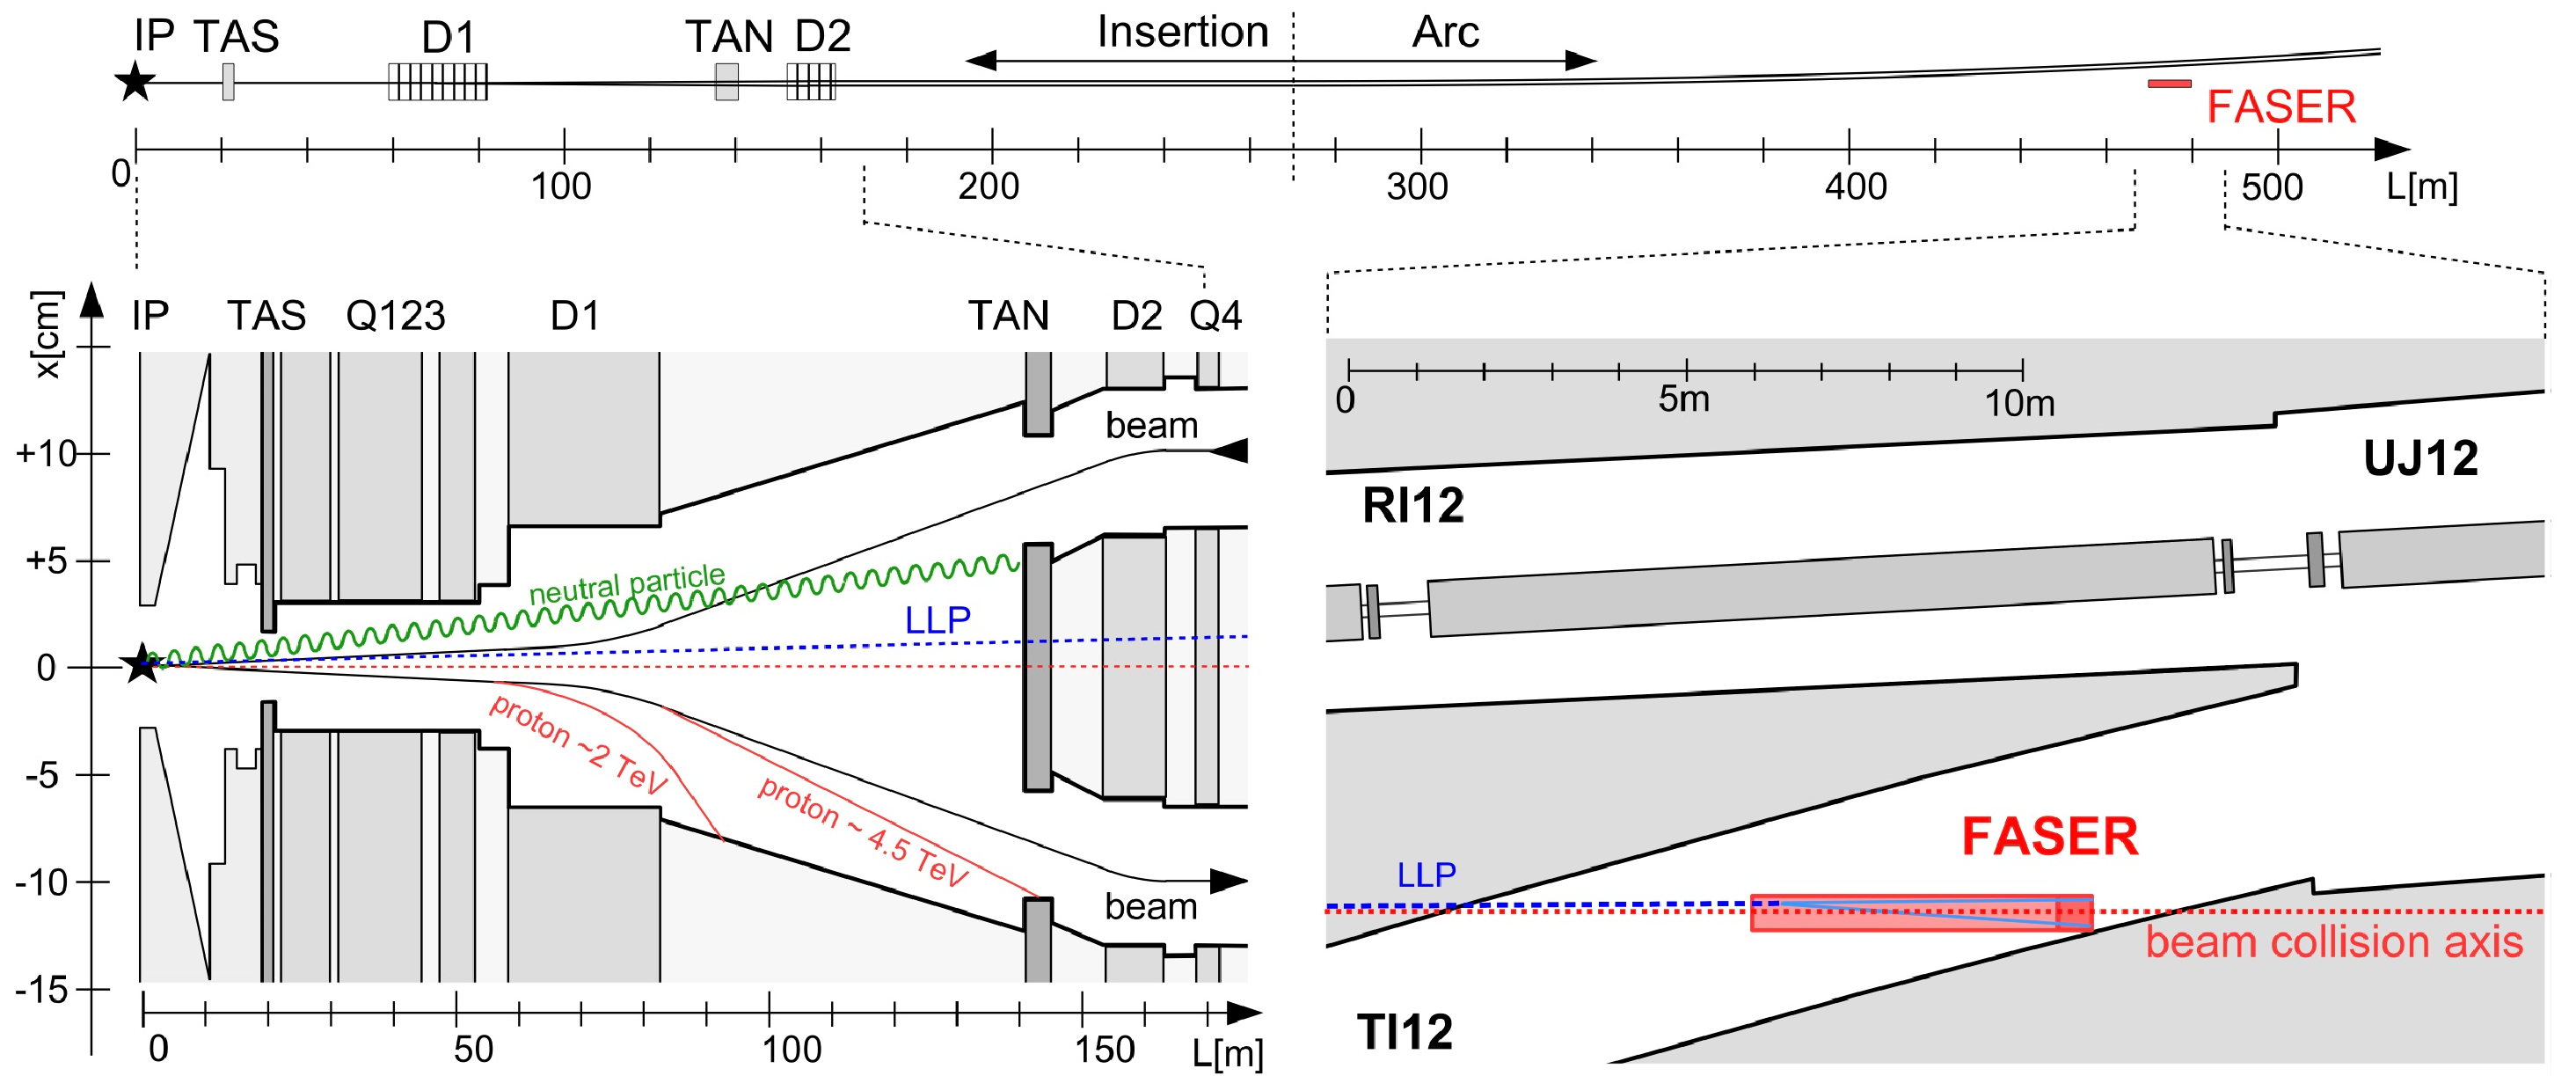
\includegraphics[width=0.9\textwidth]{files/FASER_location}
    	\caption{Location of the FASER detector in the TI12 tunnel, \SI{480}{\meter} downstream of the ATLAS IP. The beam bending in the arc creates a clear line of sight for particles produced in the far-forward region.}
    	\label{fig:faser_location}
	\end{figure}
	
	In this context, FASER serves as a complementary approach to more conventional LHC experiments. It enables probing of new regions of parameter space, particularly for low-mass, long-lived, and weakly coupled particles. Its small footprint and cost-effective design make it an attractive model for future LLP searches, and its results are expected to provide crucial insights into the hidden sector. In the following chapter at first will come a presentation of the physics potential of FASER as a probe of the hidden sector for discovery of potential DM candidates. An overview of the FASER detector along with its background from the SM and typical signatures for LLP decays. Finally, the emphasis will be put on an ALP model in which the particle is produced through rare meson decays and decays into two photon within FASER, building ground for the proposal on an upgrade of a sub-component of the original detector layout: the PreShower. 
	
	\clearpage
	
	\section{Physics program: A probe to the Hidden sector and more}
	The location of the FASER detector provides reach to a wide range of LLP models decaying into SM particles with energies in the TeV range. It also provides a novel measurement of neutrino interactions when produced at colliders. In the following section, a presentation of the different production mechanisms for LLPs as well as two leading LLP model probed by FASER will be presented, a complete overview of FASER's reach for LLPs is presented in \cite{FASER_LLP} with various benchmark models used to motivate the need for an experiment such as FASER. The motivation is further complemented through the study of neutrinos reaching FASER and equivalently, a detailed study can be found in \cite{neutrino_FASER}.  
	
		\subsection{Production of LLPs}
		Multiple production mechanisms are responsible for the production of new light particles at the LHC, including rare decays from light and heavy hadrons, dark bremsstrahlung in coherent proton-proton collisions, direct production in hard scattering: FASER being located after a neutral particle absorber (TAN), the particles created at the ATLAS Interaction Point (IP) may travel \SI{140}{\meter}, interact with the TAN and make it a beam dump experiment \cite{FASER_LLP}. The Feynman diagrams for each production mechanism are presented below and will be used along the upcoming discussion \cite{FASER_LLP}.
		\begin{figure}[h]
			\centering
			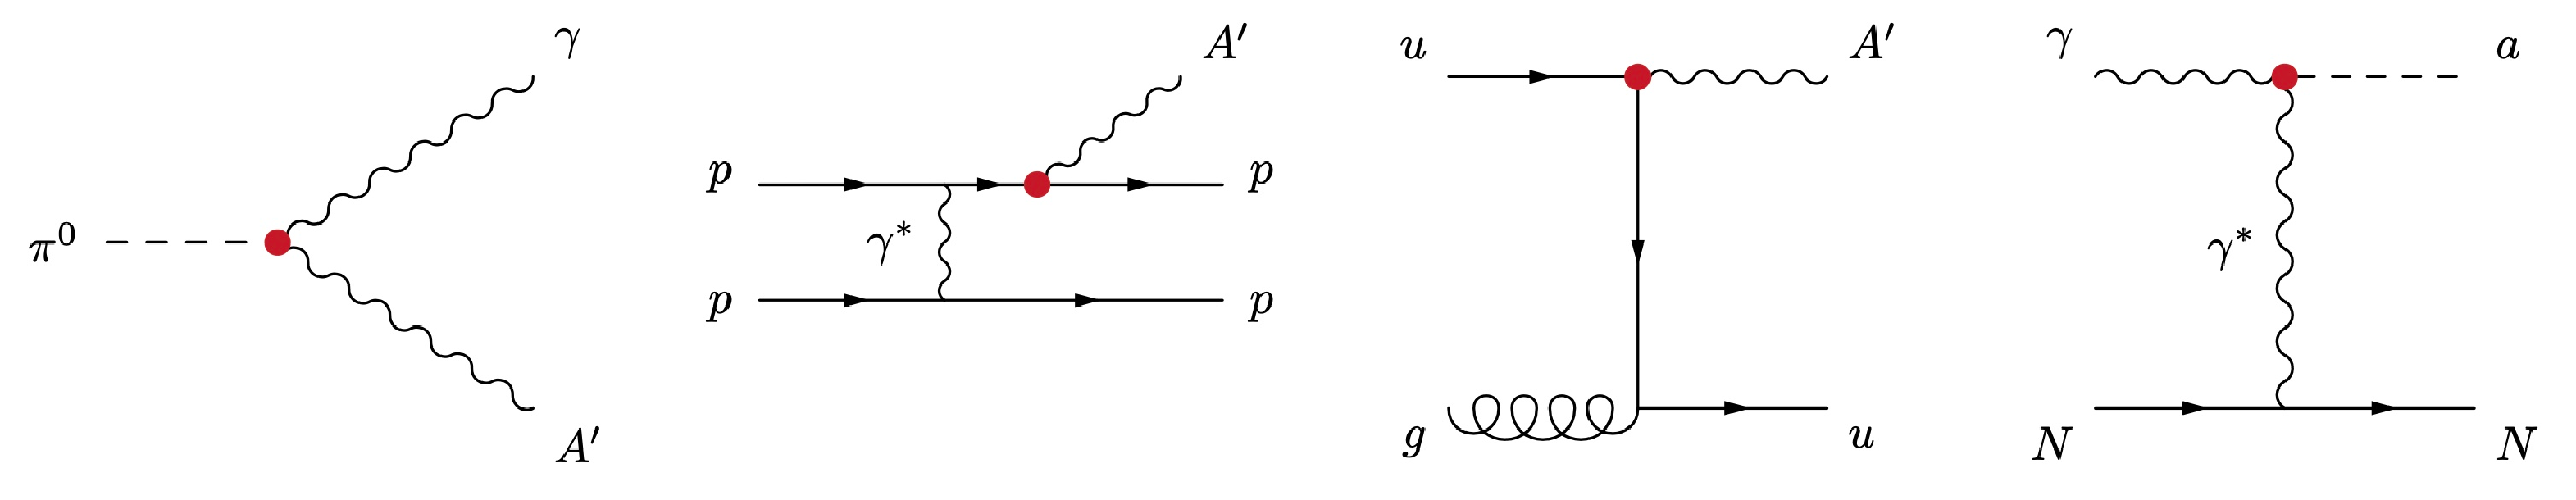
\includegraphics[width=0.95\linewidth]{files/Feynman_production_mechanism}
			\caption{From left to right, production mechanisms via: rare meson decay, dark bremsstrahlung, hard scattering and Primakoff process from photon in the TAN.}
			\label{im:prod_mech_feynman}
		\end{figure}
		\subsubsection{Rare meson decays}
		The large hadron flux from the ATLAS IP in the very forward direction makes the production of LLP coupled to quark a prominent production mechanism through rare decays into LLPs from hadrons kinematically compatible. 
	
		The flux of light hadron is mainly composed of neutral pions ($\pi^0$) and eta mesons $\eta$ with respectives cross sections of $\sigma_{\pi^0} = 1.6 \times 10^{12}$ pb and $\sigma_{\eta} = 1.7 \times 10^{11}$ pb. Alternatively, the flux of heavy hadrons mainly composed of D-mesons and B-mesons with respectives cross sections of $\sigma_{B} = 7.4 \times 10^{9}$ pb and $\sigma_{D} = 4.7 \times 10^{8}$ pb. As shown before, these particles are emitted in the very forward direction with a very small angle with respect to the beam axis. The spectrums for the production of $\pi^0$ and B-mesons in the $(\theta, p)$ plane with $\theta$ the emission angle of the meson with respect to the beam axis and $p$ their momentum is presented in the figure \ref{im:hadron_flux}  \cite{FASER_LLP}.
	 	\begin{figure}[h]
			\centering
			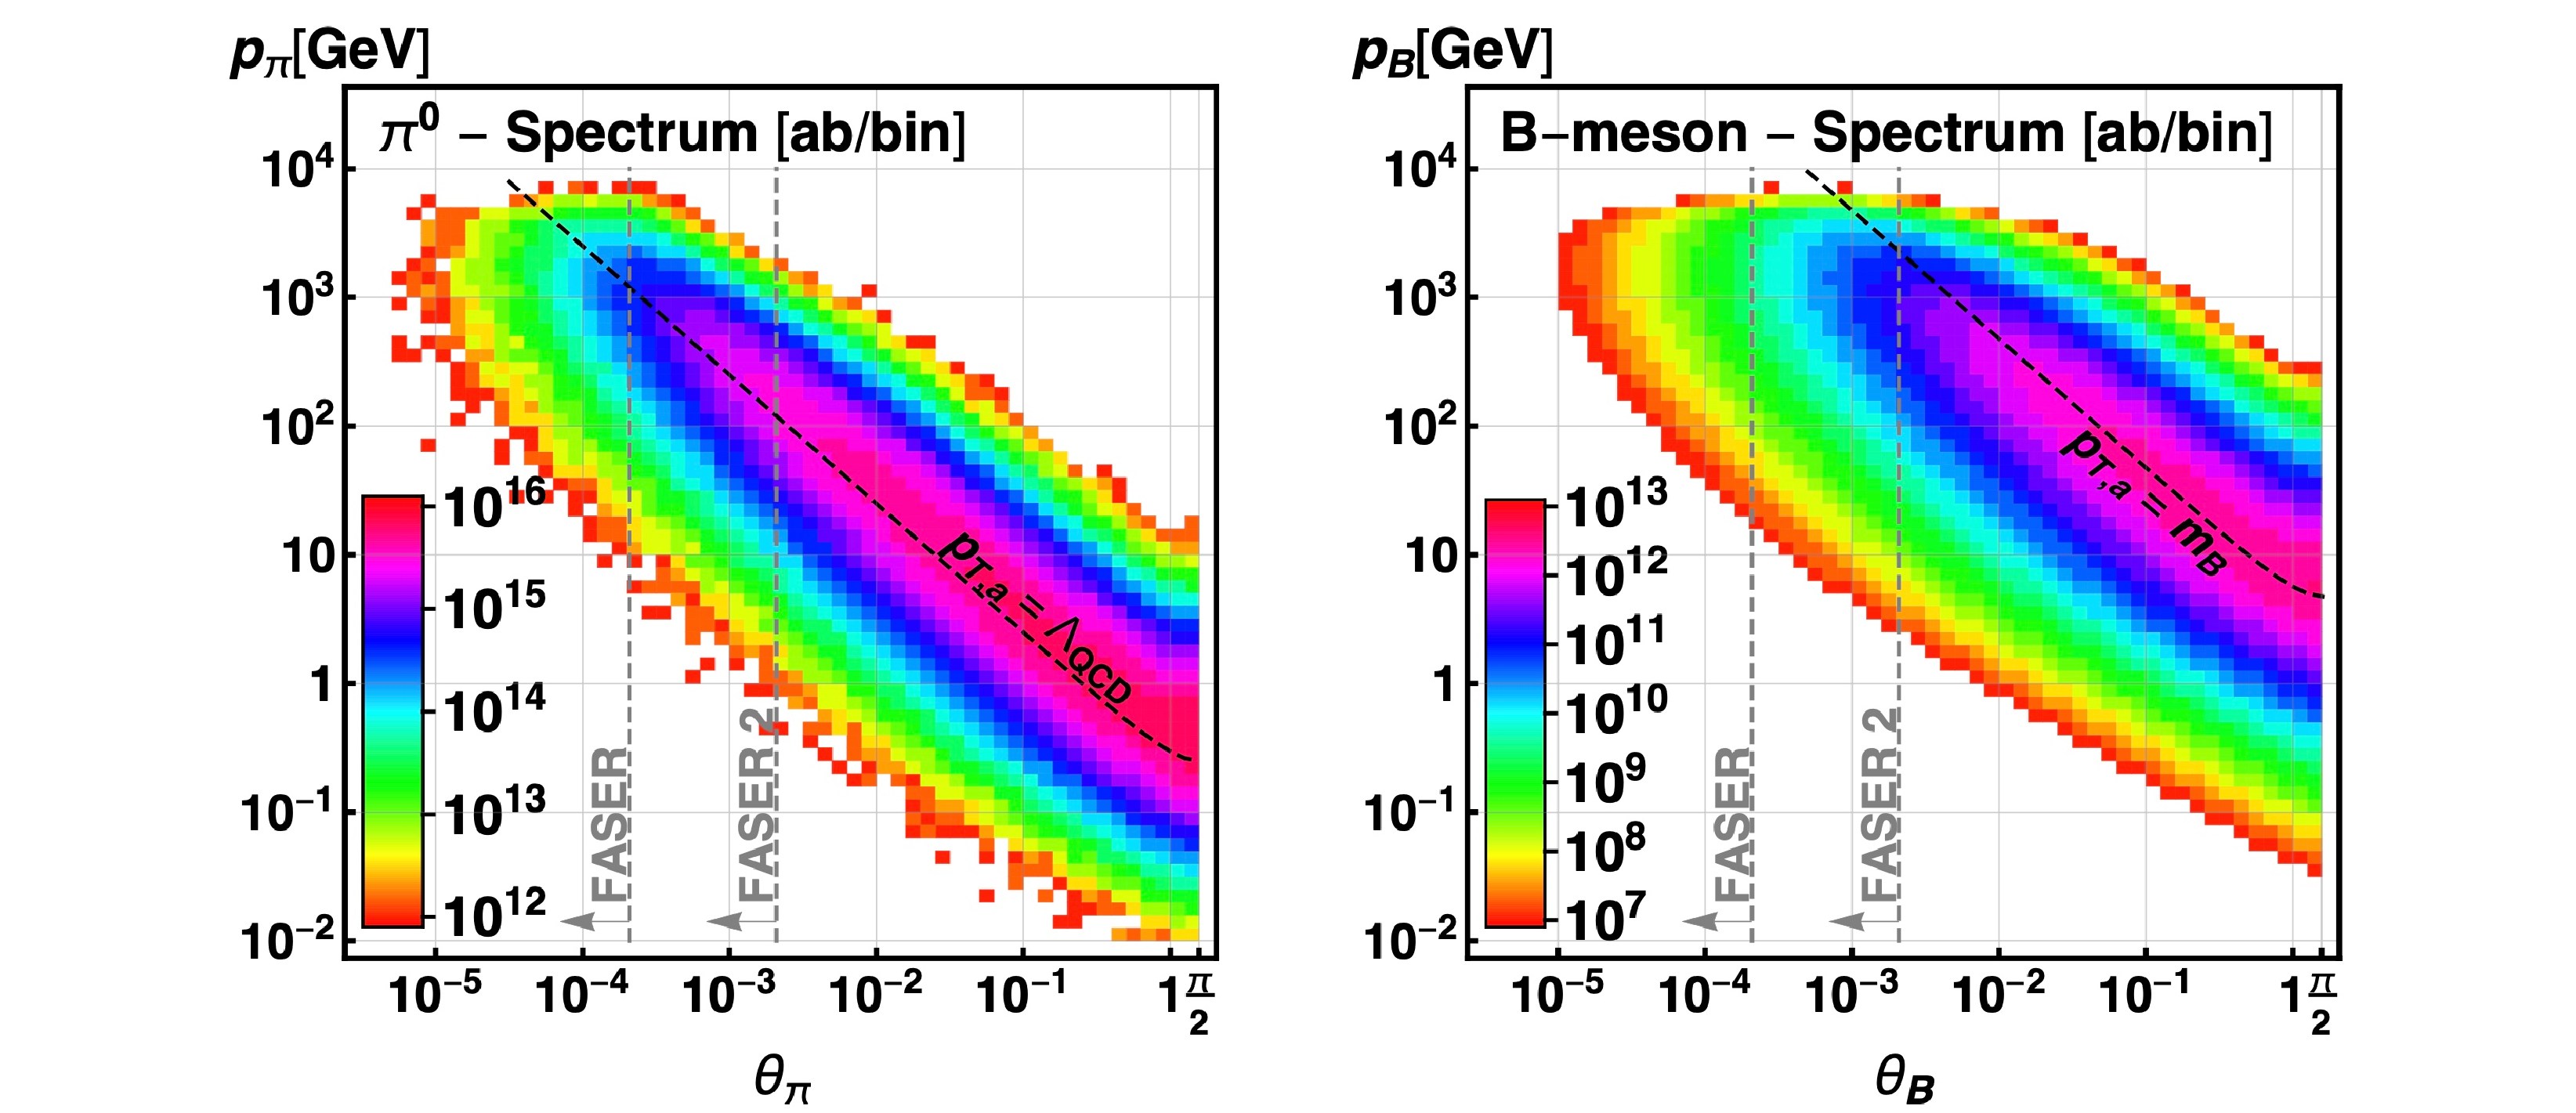
\includegraphics[width=0.95\linewidth]{files/pi0_B_meson_flux}
			\caption{Differential meson production rates in the $(\theta, p)$ plane with $\theta$ the emission angle with respect to the beam axis and $p$ their momentum. The angular acceptance of FASER and a potential upgrade, FASER2 are shown as dashed vertical grey lines.}
			\label{im:hadron_flux}
		\end{figure}

		
		\subsubsection{Dark Bremsstrahlung}
		If LLPs were to be heavier than the kinematic threshold for production via decay, their production could be dominated by what is called dark bremsstrahlung in proton-proton scattering as show in \ref{im:prod_mech_feynman}. This production is particularly relevant for dark vector bosons $V$ for masses of the LLP such that $m_V > m_\pi$. For other types of models, a different production mechanism put shade onto the dark bremsstrahlung put it sill contributes with a subdominant role. 
		
		\subsubsection{Hard scatterings}
		At the parton level, a plethora of hard scatterings between the constituents of the protons can produce LLPs as illustrated in \ref{im:prod_mech_feynman}. The large incertitudes on the parton distributions functions at low momentum transfer makes an accurate LLP production rate estimation difficult through this channel \cite{FASER_LLP}. On the contrary, if the mass of the LLP would be such that $M_{LLP} >$ \SI{2}{\giga\electronvolt}, the Drell-Yann process could become dominant as discussed in \cite{Drell_Yann}. In what follows, this production mechanism will not be considered. 
		
		\subsubsection{"Beam Dump" production}
		
		The large number of particles produced in the very forward region that can travel \SI{140}{\meter} before interacting with the TAN produces a fixed-target beam dump experiment able to produce LLPs. One particularly dominant process is the Primakoff process for which photons copiously produced at the ATLAS IP interact with the TAN and produce an LLP as show in \ref{im:prod_mech_feynman}. Figure \ref{im:photon_ATLAS_ALP} (left panel) shows the spectrum for production of photon from the ATLAS IP. The acceptance of the TAN set a constraint at the level of $\theta_a < 10^{-3}$ for photons to interact \cite{Primakoff_process}. Similarly, dark vector bosons $V$ could be produced via dark Compton scattering ($ \gamma e^- \rightarrow V e^-$) but this process remains subdominant with respect to other production mechanisms. 
	
		
		\subsubsection{LLPs reaching FASER}
		Once produced, an LLP of mass $m$  with an angle $\theta$ and momentum $p$ with respect to the beam axis, has a probability of decaying within FASER given by geometrical acceptance such that: 
		\begin{equation}
			\mathcal{P}(\theta, p) = {\left( e^{-(L-\Delta)/d} - e^{-L/d}\right)} \hspace{1mm} \Theta \left(R-L\tan(\theta)\right) \approx \frac{\Delta}{d}e^{-L/d} \hspace{1mm} \Theta \left(R-L\tan(\theta)\right)
		\end{equation}
		where $L$ denotes the distance between IP and FASER, $R$ the radius of the detector and $\Delta$ the length of the decay volume. The variable $d$ is defined as the decay length of the LLP in the lab frame and can be written as $d = c \tau \beta \gamma$ with $\tau$ the LLP's lifetime. The number of LLPs decaying inside FASER can then be written as \cite{FASER_LLP}: 
		\begin{equation}
			N_{\text{LLP decay}} = \mathcal{L} \int dp \hspace{1mm} d\theta \frac{d\sigma_{pp \rightarrow LLP + X}}{dp \hspace{1mm} d\theta} \cdot \mathcal{P}(\theta, p)
		\end{equation}
		
		In the following discussion for different benchmark models in the physics reach of FASER, the decay of LLP into invisible dark sector particles will be neglected so that only detectable event rate can be quoted. Additional contributions such as detection efficiency will be neglected and set at 100 \% for the ease of comparison with other experiments. 
		
		
		\subsection{Vector Portal: Dark photon}
		On of the best motivated LLP model includes the addition of a U(1) symmetry with renormalizable coupling and the corresponding vector field $X_\mu$ coupling through kinetic mixing to the SM hypercharge gauge bosons  or at low energies to the SM photon \cite{FASER_LLP}. The dark photon model emerges from this completion of the SM and the Lagrangian is extended as: 
		\begin{equation}
			\mathcal{L} = \mathcal{L}_{SM} + \frac{1}{2} m'^2X^2 - \frac{\epsilon'}{2}F_{\mu \nu}F'^{\mu \nu}
		\end{equation} 
		
		where $\epsilon'$ parametrises the kinetic mixing term and $F_{\mu \nu}$ and $F'^{\mu \nu}$ are the field strength tensor of the SM photon and $X$ the one of the new gauge boson. After rotation into the mass basis, the photon-SM fermion coupling parameter is given by $\epsilon = \epsilon' \cos{\theta_W}$. Removing the kinetic mixing term after a field re-definition, the dark photon field $A'$ emerges as a physical mass eigenstate coupling to charged SM fermions through their electric charge so that \cite{FASER_LLP}: 
		
		\begin{equation}
			\mathcal{L} = \mathcal{L}_{SM} + \frac{1}{2} m_{A'}^2A'^2 - \epsilon e \sum_f q_f \bar{f} \gamma_\mu A'^\mu f 
		\end{equation} 
		
		where $g_f$ is the charge of the fermions and $f$ (and $\hat{f}$) the field of the fermions themselves. As discussed before, the dark photon may be produced both through rare decays of light mesons (at low values of $m_{A'}$) like $\pi , \eta \rightarrow \gamma A'$ and also at higher masses predominantly by dark bremsstrahlung. These processes are neglected with respect to the SM counterparts roughly by a factor $\epsilon^2$ \cite{FASER_LLP}. \\ 
		
		Once produced, the dark photon may decay into a pair of charged leptons, for the smallest masses to a $e^+ \hspace{1mm} e^-$ pair if $m_{A'} > 2m_e$ and other heavier pairs, even hadronic if the kinematic conditions are met.The partial decay width for the dark photon into an $e^+ \hspace{1mm} e^-$ pair is given by \cite{dark_photon_Feng} : 
		\begin{equation}
			\Gamma (A' \rightarrow e^+ \hspace{1mm} e^-) = \frac{\epsilon^2 e^2 m_{A'}}{12 \pi} \left[ 1-\left( \frac{2m_e}{m_{A'}} \right)^2 \right]^{1/2} \left[ 1 + \frac{2m_e^2}{ma_{A'}^2} \right] 
		\end{equation}
		The total dark photon decay width can then be obtained through the use of the branching ratio of dark photon into $e^+ \hspace{1mm} e^-$ pair $\mathcal{B}(A' \rightarrow e^+ \hspace{1mm} e^-)$ so that it reads: 
		\begin{equation}
			\Gamma_{A'} = \frac{\Gamma (A' \rightarrow e^+ \hspace{1mm} e^-)}{\mathcal{B}(A' \rightarrow e^+ \hspace{1mm} e^-)}
		\end{equation}
		In the limit in which $E_{A'} \gg m_{A'} \gg m_e$ the dark photon decay length can then be written as: 
		\begin{equation}
			\bar{d}_{A'} = c \frac{1}{\Gamma_{A'}} \gamma_{A'} \beta_{A'} 
%			\approx \text{(80 m)} \mathcal{B}(A' \rightarrow e^+ \hspace{1mm} e^-) {\left[ \frac{10^{-5}}{\epsilon} \right]}^2 {\left[ \frac{E_{A'}}{\text{TeV}} \right]} {\left[ \frac{100 \text{ MeV}}{m_{A'}} \right]}^2
		\end{equation}
		
		The dark photon decay length, branching fractions into leptonic and (heavier) hadronic states are shown in the left panel of figure \ref{im:dark_photon_prod}. The sensitivity reach in the $m_{A'}$ and $\epsilon$ parameter space for FASER for dark photons is presented in the right panel of figure \ref{im:dark_photon_prod} together with a comparison between the already excluded regions (in grey), current and future experiments.
		\clearpage
		\begin{figure}[h]
			\centering
			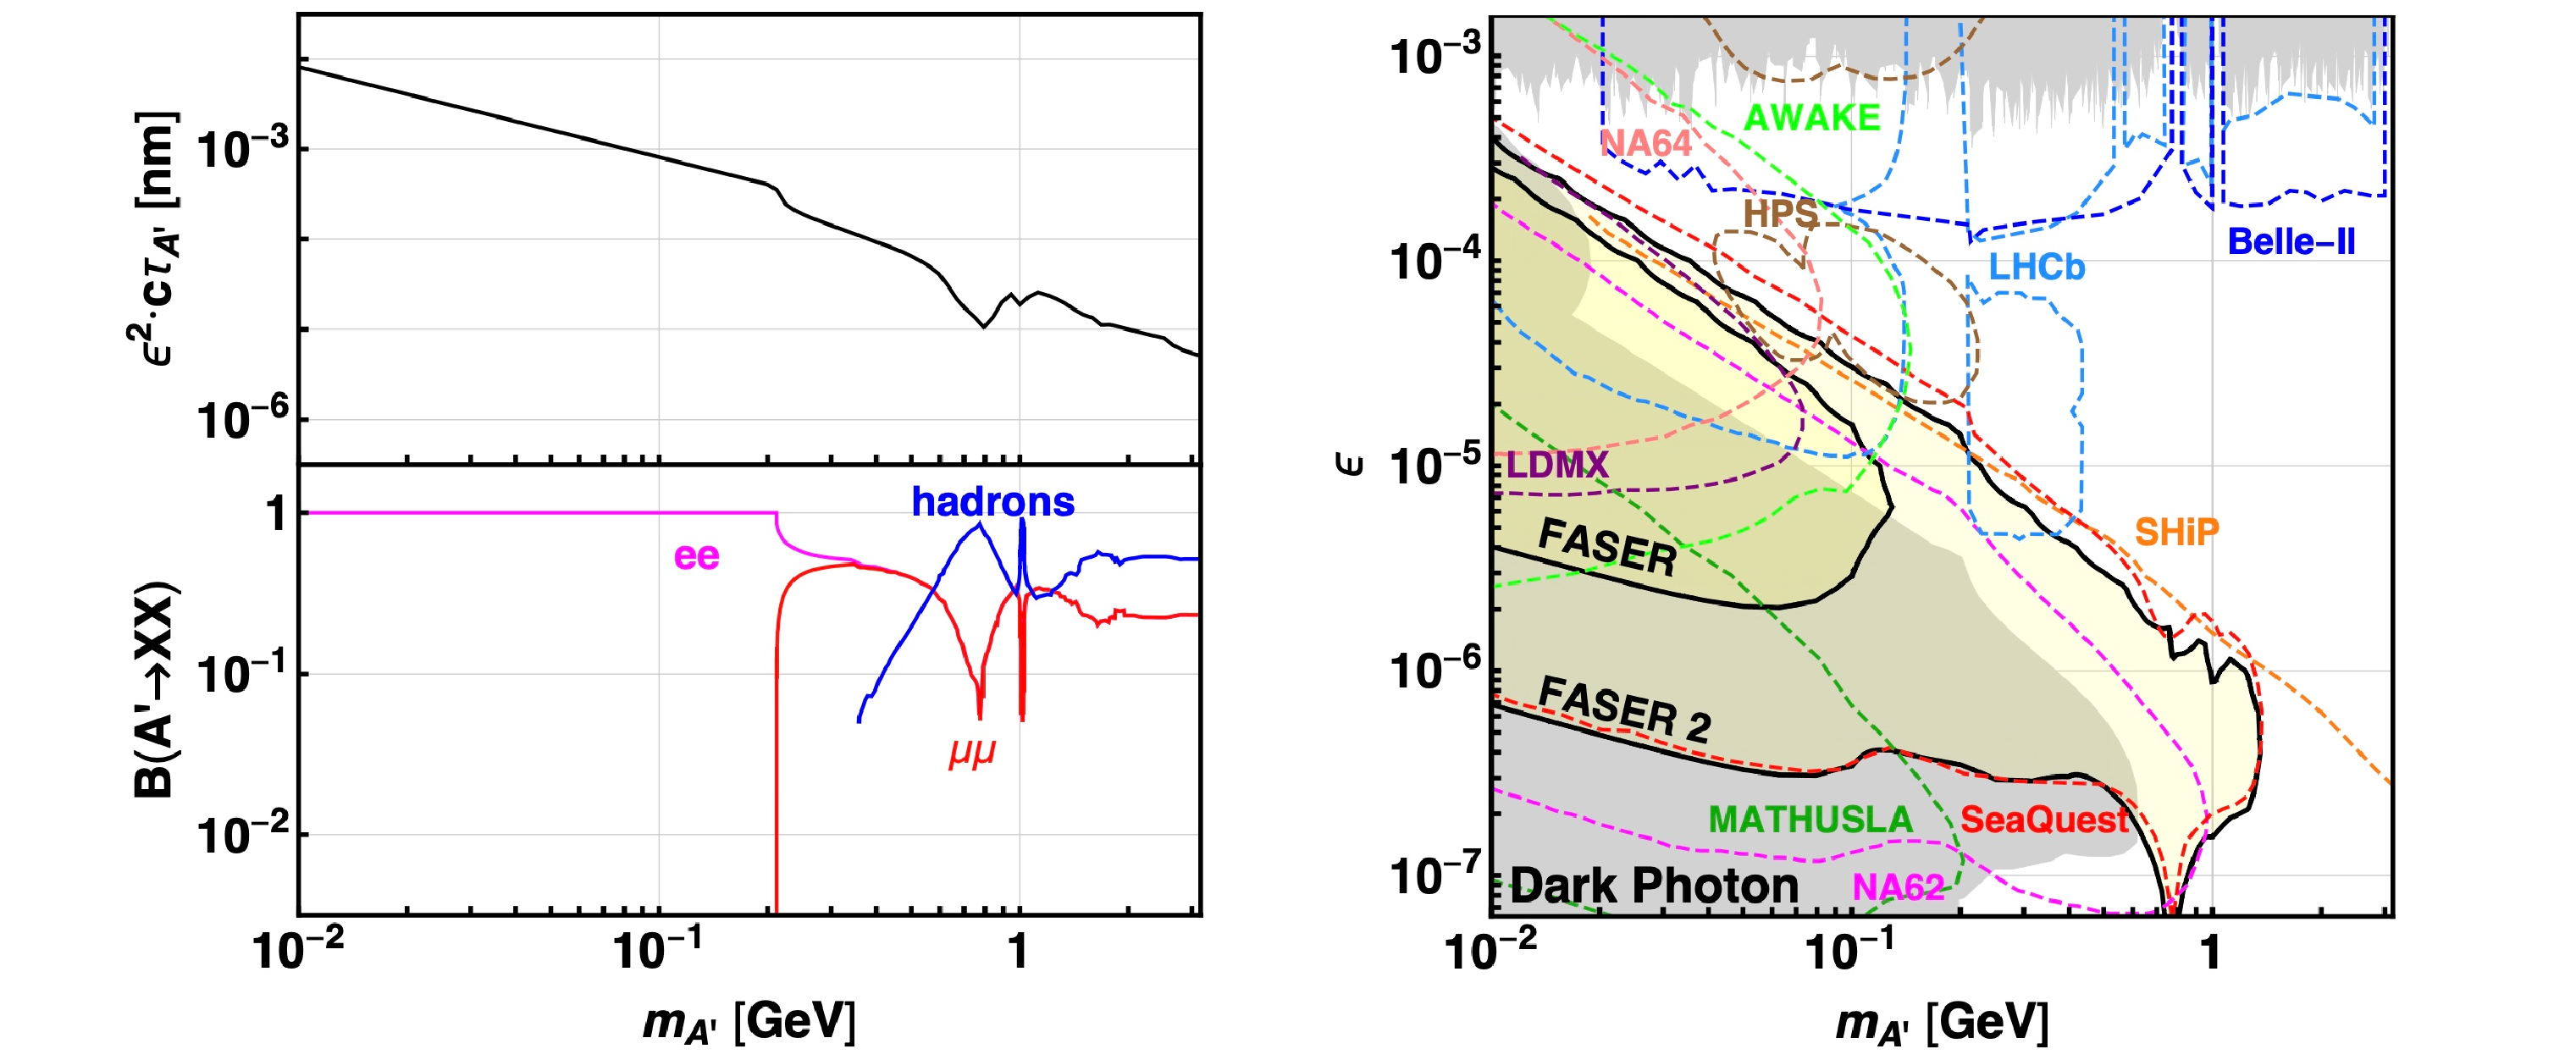
\includegraphics[width=0.95\linewidth]{files/dark_photon_production}
			\caption{The dark photon decay length (top left panel), its branching fractions in diverse possible final states (bottom left panel) and FASER's reach in the dark photon parameter space defines by its mass and kinetic mixing parameter}
			\label{im:dark_photon_prod}
		\end{figure}
		
		A detailed interpretation of the sensitivity reach presented is given in \cite{FASER_LLP} but is is striking to see that FASER will already be able to probe an interesting section of the parameter space throughout the LHC Run 3. The boundary at very low mixing parameter is given by the $\epsilon^4$ dependence of both production and decay mechanisms, both happening through the mixing of the dark photon to SM fermions. On the other hand, the boundary for high mixing parameter becomes exponentially suppressed as the dark photon will decay before even reaching the detector \cite{FASER_LLP}.  
		
		
		\subsection{Pseudoscalar Portal: Axion Like Particles}
		
		Axion-Like-Particles differ from other models through the dimension-5 operators through which they couple to the SM. They manifest themselves as pseudo Nambu-Goldstone bosons arising from the spontaneous breaking of a global symmetry. A more detailed explanation of the motivation behind the ALP model will later be given in section \note{cite section}. In the most general form of ALP models, it couples to photons, gluons and fermions and a a general extension of the Sm Lagrangian is given by: 
		\begin{equation}
			\mathcal{L} = \mathcal{L}_{SM} + -\frac{1}{2} m_a^2 a^2 - \frac{1}{4} g_{a\gamma\gamma} a F_{\mu\nu} \tilde{F}^{\mu\nu} - \frac{g_s^2}{8} g_{agg} a G_{\mu\nu}^A \tilde{G}^{A\mu\nu} - i \sum_f g_{aff} \frac{m_f}{v} a \bar{f} \gamma_5 f
		\end{equation}
		
		The mass of the ALP was introduced as $m_a$ along with its coupling to photon $g_{a\gamma\gamma}$, to gluons $g_{agg}$ and to fermions $g_{aff}$. An attentive eye would have noticed that no coupling to the weak interactions gauge bosons was explicitly written, this discussion is reserved to the discussion in \note{cite section}. Since the ALP model works as an effective field theory, there is a specific energy scale $\Lambda$ at which the global symmetry is broken so that dimension-r operators are suppressed for energy values below this scale. The running of the coupling constants is defined through all of the scale coefficients for the different coupling to the SM particles ($f_\gamma$, $f_G$ and $f_f$). 
		
		For simplicity the discussion will only focus for the moment on the coupling to photons only both for the production mechanism but also for the decay of the ALP. Another production mechanism will although be presented more in details in section \note{cite section}. In this situation the photon coupling simply reduces to $g_{a \gamma\gamma} = 1/f_\gamma$ up to some scale after which corrections are required. The ALP also inherits loop-induced couplings to fermions but are suppressed and are typically negligible. The Lagrangian then reduces to the following form: 
		\begin{equation}
			\mathcal{L} = \mathcal{L}_{SM} - \frac{1}{2} m_a^2 a^2 - \frac{1}{4} g_{a\gamma\gamma} a F_{\mu\nu} \tilde{F}^{\mu\nu}
		\end{equation}
		As discussed before, the ALP when coupled to photon will predominantly be produced through rare decays of light mesons, and the Primakoff process \cite{ALPTraum} which becomes the major contribution for ALP with significant boost in the very forward direction due to the copious flux of photons coming from the ATLAS IP as shown in figure \ref{im:photon_ATLAS_ALP} (left panel). \\ The spectrum ifor photon interacting in the TAN and producing ALPs (center panel) and for ALPs decaying within FASER (right panel). 
		\begin{figure}[h]
			\centering
			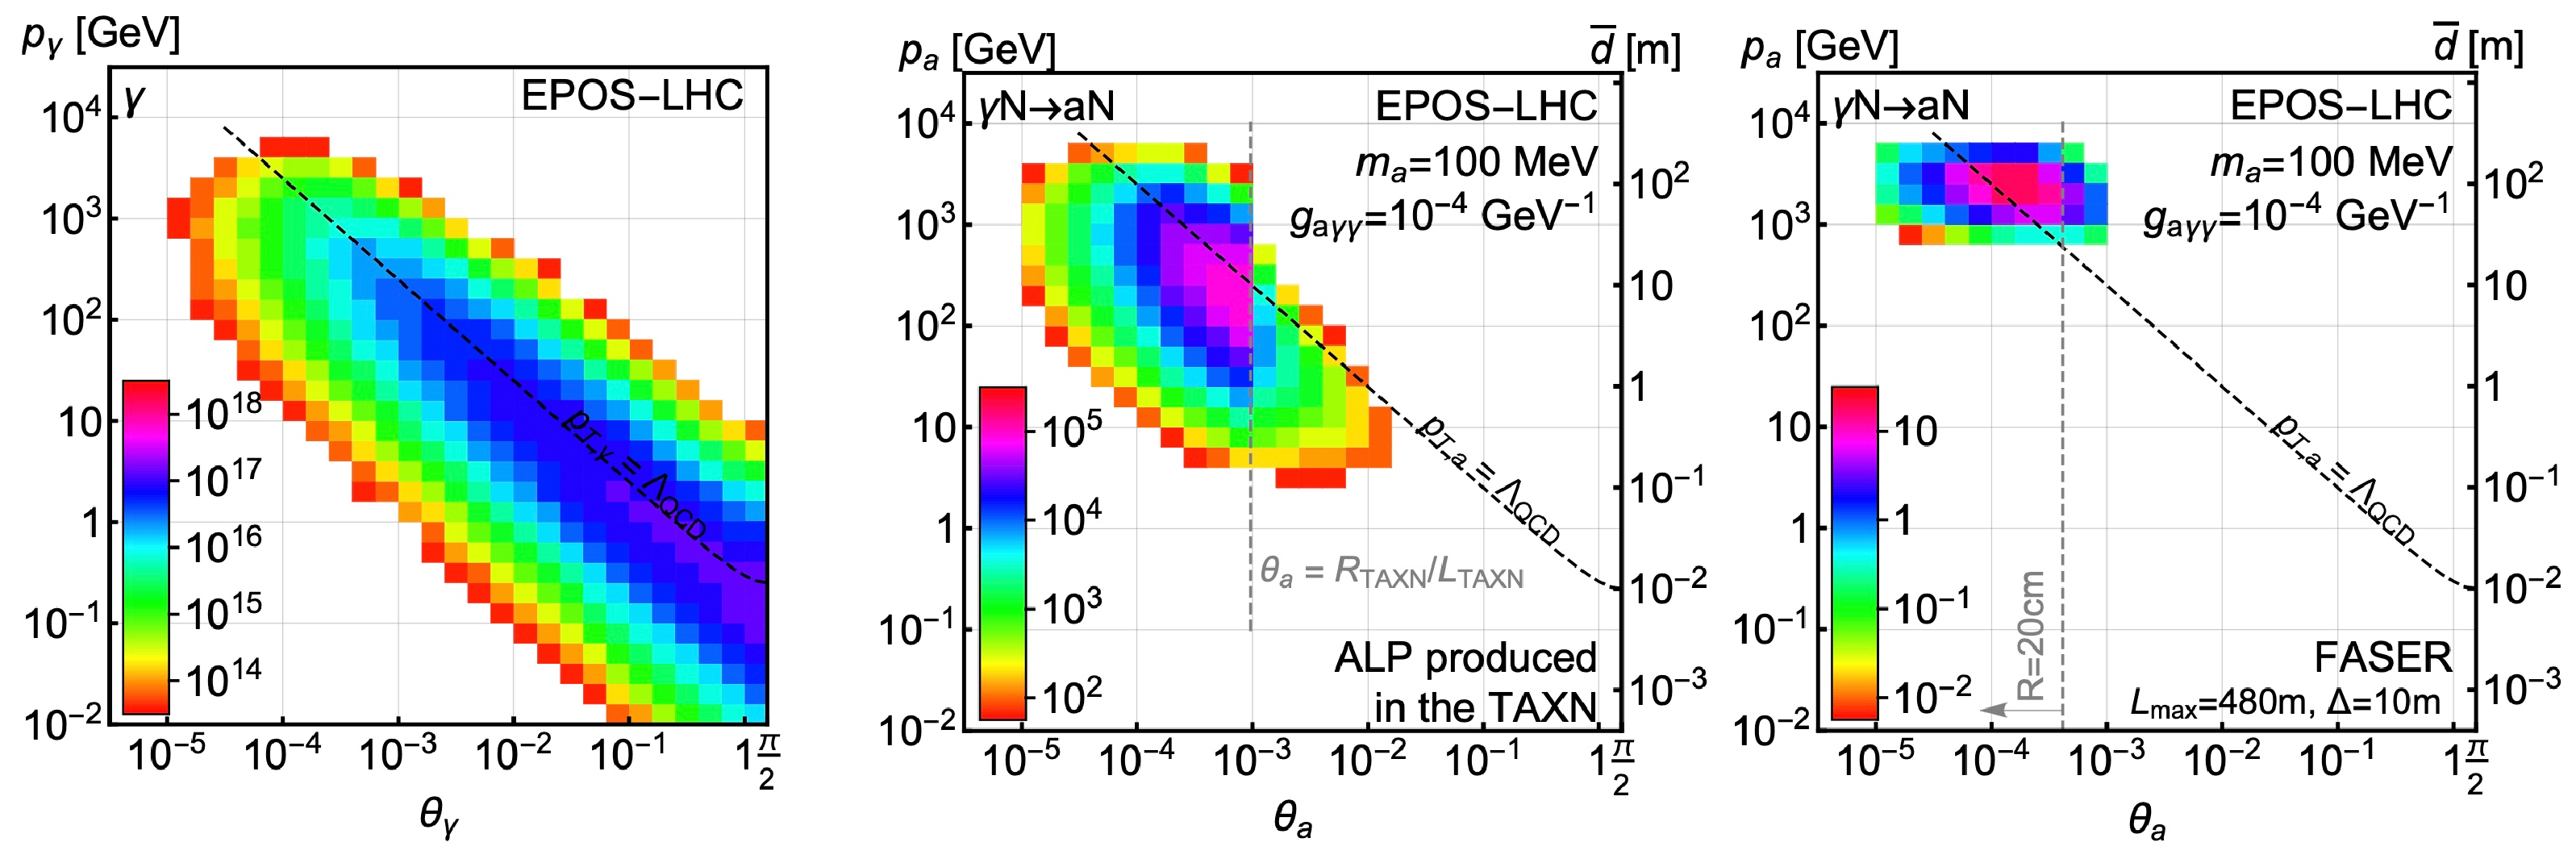
\includegraphics[width=0.95\linewidth]{files/primakoff_prod_TAN}
			\caption{Originating from the photon flux from ATLAS IP (left panel), ALPs can be produced in the TAN (center panel) and later reach FASER and decay (right panel)}
			\label{im:photon_ATLAS_ALP}
		\end{figure}
		
		Once produced, the ALPs will mainly decay into a pair of photons as the decay into fermions pair is suppressed in this reduced model with only photon coupling at leading order. One of the sub-leading decays channel is the one in which the ALP decays into one real and one virtual photon, further decaying into an electron-positron pair with a branching fraction of the order of $\mathcal{B}(a \rightarrow \gamma e^+ \hspace{1mm} e^-) \approx 1 \%$ \cite{FASER_LLP}. For the primary ALP decay channel, the decay width is given by: 
		\begin{equation}
			\Gamma_a(a\rightarrow \gamma \gamma) = \frac{g_{a \gamma\gamma}^2 m_a^3}{64 \pi}
		\end{equation}
		
		The cubic dependence on the mass of the ALP is a consequence of the dimension-5 operator which mediates the di-photon coupling. The decay length of the ALP can then be written as: 
		\begin{equation}
			\bar{d}_a = c \frac{1}{\Gamma_{a}} \gamma_{a} \beta_{a} 
			\label{eq:ALP_decay_length}
		\end{equation}
		
		The ALP decay length, branching fractions into di-photon and sub-leading fermionic channel are shown in the left panel of figure \ref{im:ALP_photon_prod}. The sensitivity reach in the $m_{a}$ and $g_{a\gamma\gamma}$ parameter space for FASER for ALPs produced through Primakoff Process is presented in the right panel of figure \ref{im:ALP_photon_prod} together with a comparison between the already excluded regions (in grey), current and future experiments.
		
		A detailed interpretation of the sensitivity reach presented is given in \cite{FASER_LLP} but is is striking to see that FASER will already be able to probe unconstrained regions with potential discovery in the mass range $m_a  \sim $ 30 - \SI{400}{\mega\electronvolt} throughout the LHC Run 3 \cite{Primakoff_process}. For large couplings to di-photon, the sensitivity reach is constrained by the decay length of the ALP while for lower couplings the lifetime is usually longer as ALPs are less boosted, resulting in a larger emission angle with respect to beam axis for which the geometrical acceptance of the detector becomes the limiting factor \cite{Primakoff_process}. 
		\clearpage	
		
		\begin{figure}[h]
			\centering
			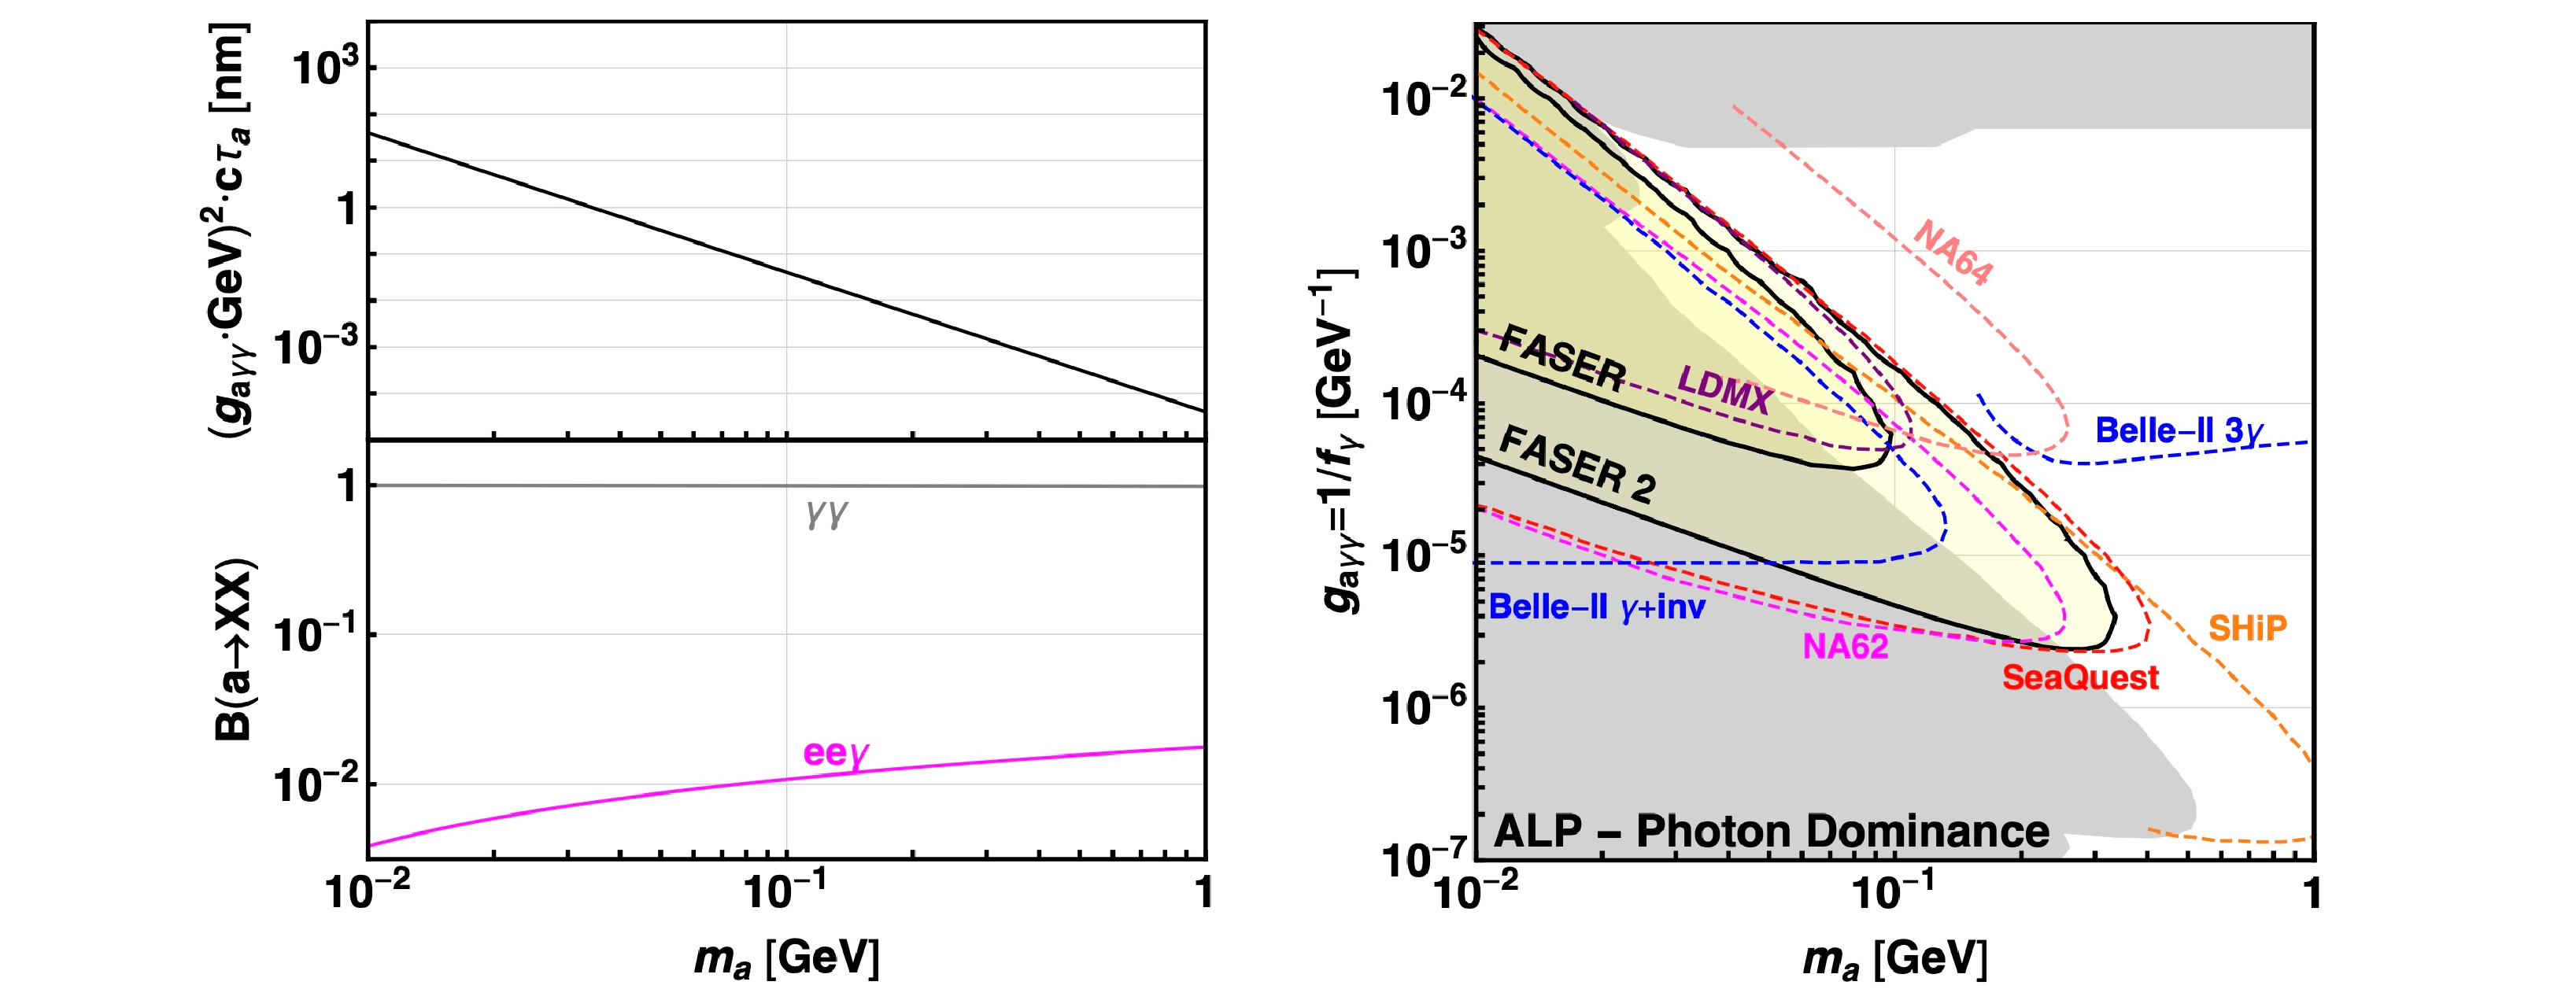
\includegraphics[width=0.9\linewidth]{files/ALP_photon_production}
			\caption{The ALP decay length (top left panel), its branching fractions in diverse possible final states (bottom left panel) and FASER's reach in the ALP parameter space defines by its mass and coupling to di-photons}
			\label{im:ALP_photon_prod}
		\end{figure}
		
			
		\subsection{Neutrinos from collider}
		The special location of the FASER detector doesn't only provide good sensitivity to BSM model but also provides a completely new way of studying neutrinos from collider experiments. The large flux of hadrons in the very forward direction produces through their decay a significant flux of neutrinos highly collimated along the beam axis. All three flavours of neutrinos will be able to reach FASER, if one was to assume a detector with target mass \SI{1.1}{\tonne} (FASER$\nu$) exposed to an integrated luminosity of 150 fb$^{-1}$, the number of neutrinos reaching FASER, undergoing Charged-Current (CC) interactions and their average energy deposition would be those found in Table \ref{tab:neutrinos_flux}.
		\begin{table}[h]
    		\centering
    		\begin{tabular}{|l|c|c|c|}
        		\hline
        		& $\nu_e$ & $\nu_\mu$ & $\nu_\tau$ \\
       		 	\hline
       		 	Dominant production process & $K \to \nu_e e X$ & $\pi \to \nu_\mu \mu$ & $D_s \to \nu_\tau \tau$ \\
        		\hline
        		Number of $\nu$ traversing FASER$\nu$ & $3 \times 10^{11}$ & $2 \times 10^{12}$ & $8 \times 10^{9}$ \\
        		\hline
        		Number of $\nu$ interacting in FASER$\nu$ (1.1 tonnes) & 830 & 4400 & 14 \\
        		\hline
        		Average energy of interacting neutrinos (GeV) & 820 & 820 & 810 \\
        		\hline
    		\end{tabular}
    		\caption{Expected neutrino fluxes, interactions, and average energies at FASER$\nu$ \cite{FASER_Detector}}
    		\label{tab:neutrinos_flux}
		\end{table}  
		
		\begin{figure}[h]
			\centering
			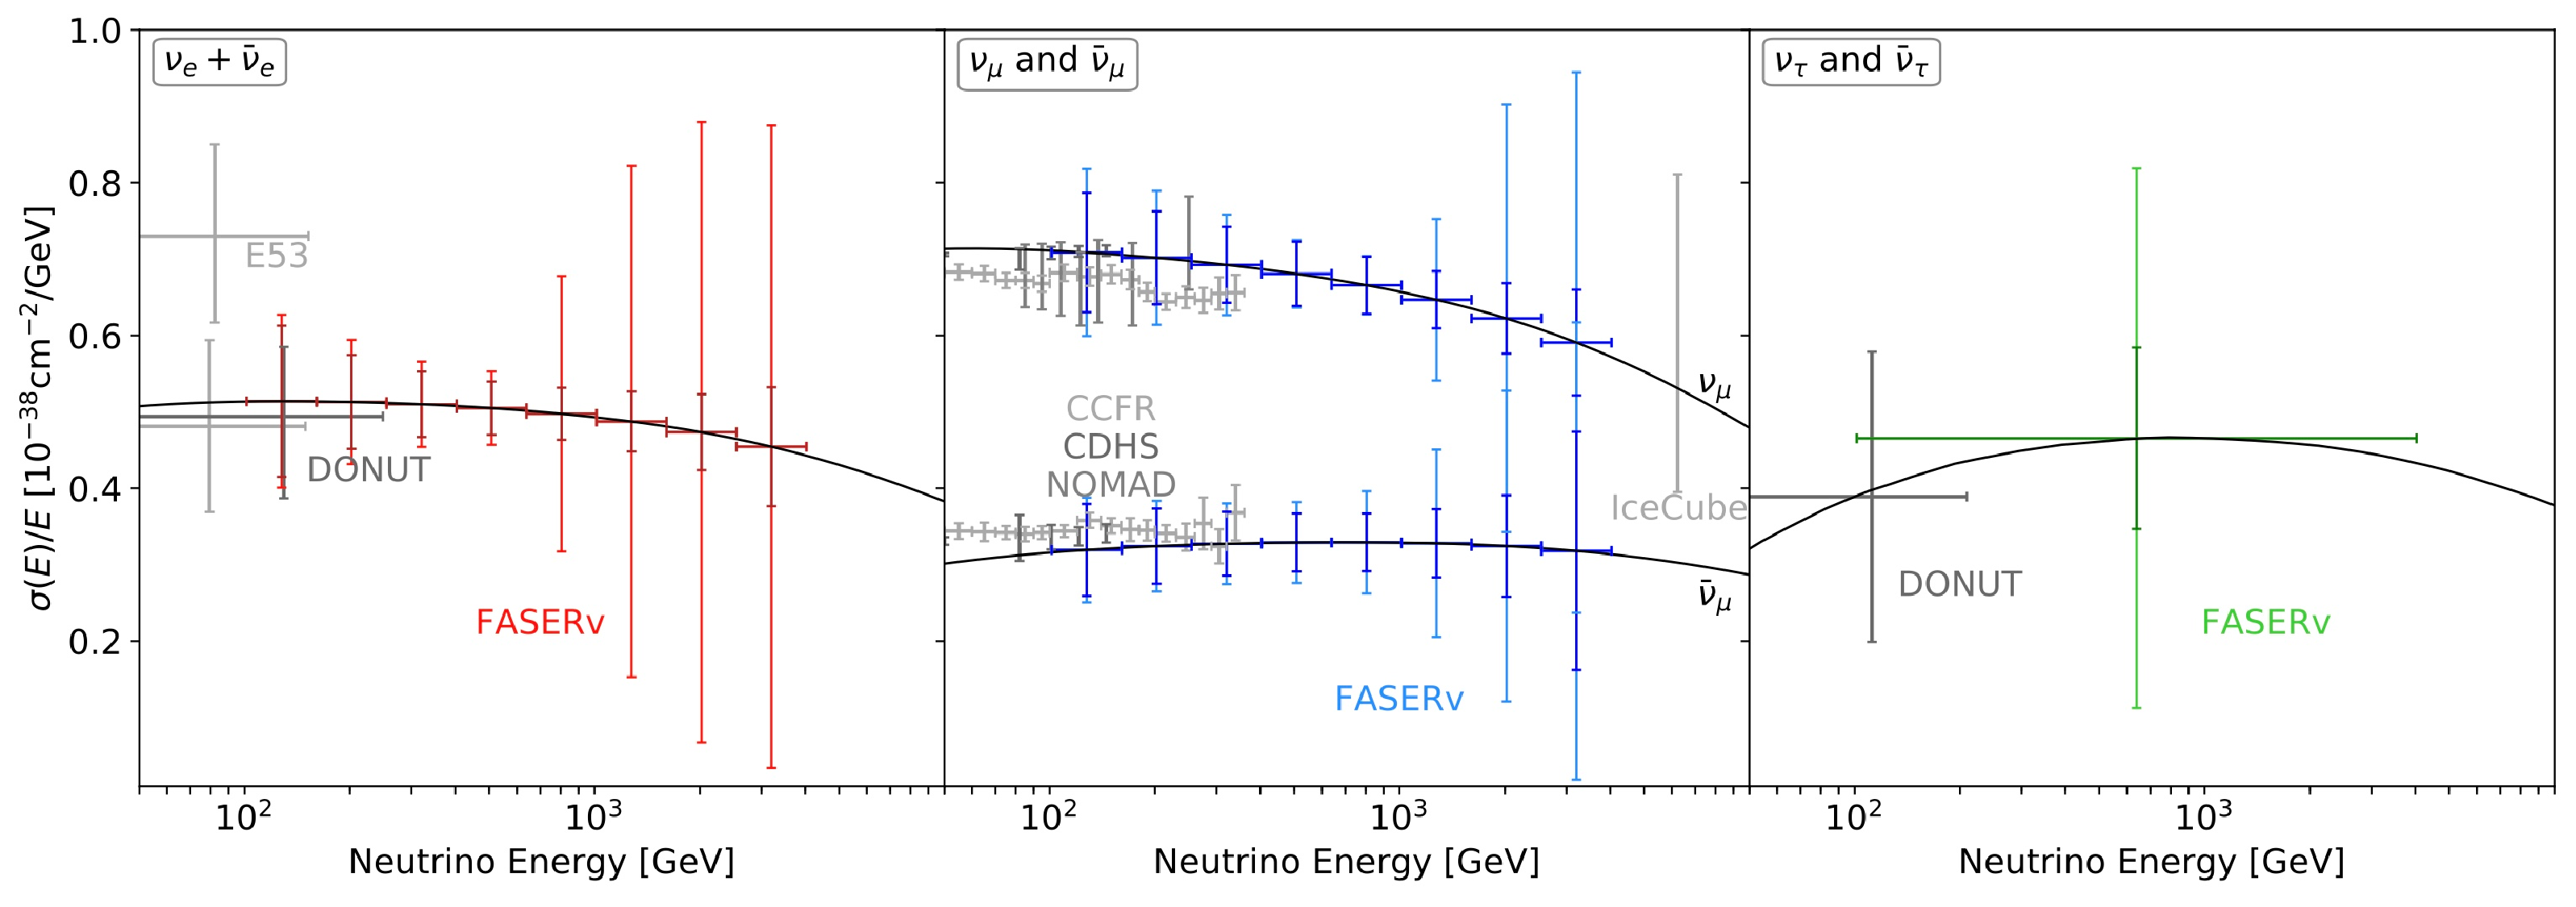
\includegraphics[width=0.845\linewidth]{files/neutrino_XS}
			\caption{FASER$\nu$ estimated CC cross section sensitivity for $\nu_e$ (left), $\nu_\mu$ (center), $\nu_\tau$ (right). The black curve is the theoretical prediction while coloured error bars are statistical uncertainties (inner) and the combination of statistical and flux uncertainties (outer).}
			\label{im:neutrino_XS}
		\end{figure}
		\clearpage
		
		Studying the flux of neutrinos reaching FASER is essential as for now, the theoretical uncertainties on the production of forward hadrons are large. As a matter of fact, varying the generator model in simulations can lead to substantial changes in the neutrino flux \cite{FASER_Detector}. A precise measurement as a function of energy and rapidity will help defining better constrains models for forward hadron production and also many more parameters as explained in detail in \cite{FASER_Detector}.  
		
		The large flux of neutrinos will allow FASER to perform a measure of the CC neutrino cross section at energy regimes not yet studied, the projection on the measurement precision is given in figure \ref{im:neutrino_XS}. The uncertainties are given separately for different generators models. 
		
		As a proof of principle, a small emulsion detector with target mass of \SI{11}{\kilo\gram} was placed along the Line of Sight (LoS) for 4 weeks during the LHC Run 2 in 2018 and recorded the first neutrino interactions candidates at a particle collider \cite{neutrino_pop}
	\clearpage
	
	
	
	\section{The ForwArd Search ExpeRiment}
	 The Physics program of FASER is quite diverse, probing both the SM in yet uncovered regimes and the hidden sector through the SM decay of LLPs originating from SM particles produced in the very forward direction at the ATLAS IP. In order to perform these various measurement, the layout of the FASER detector has to be tuned to provide the best sensitivity to the diverse signal's signatures. 
	 In the following section discussion on the possible backgrounds for the different signatures will be presented, followed by a list of the requirements on the design of the detector. An overview of the chosen layout of the detector and its subcomponents will be presented along with a brief description of the typical signatures from LLPs, shining light on the need for an upgrade of the initial detector layout to further improve sensitivity.   
	
		\subsection{Background from the Standard Model to LLP signals}
	
		Only a limited set of Standard Model particles produced at the IP can penetrate the material separating the ATLAS and FASER, made by approximately \SI{90}{\metre} of rock, concrete, and diverse infrastructures. A detailed studying FLUKA and GEANT4 simulations~\cite{FASER_techprop, FASER_loi} show that only high-energy muons and neutrinos are capable of traversing the shielding material and produce appreciable rates at FASER. The studies were made for the TI18 tunnel (opposite location to TU12 tunnel with respect to ATLAS) but there is a priori no major difference on the results \cite{FASER_techprop}. These particles constitute the dominant potential backgrounds for LLPs searches with FASER.

			\subsubsection{Muon-induced backgrounds}  
			The muons flux is predominantly produced from decay of pions, kaons and other heavy flavour hadrons produced at the ATLAS IP, the pions are mostly coming from collisions debris interacting with the LHC infrastructure such as the TAN neutral absorber. \cite{FASER_Detector}. A sub-leading source of muons actually come from the ATLAS IP itself but only account for a few percent of the total flux \cite{FASER_techprop}. The results from the FLUKA simulations predict a peak muon fluence at FASER around $\sim$ \SI{100}{\giga\electronvolt} as show in figure \ref{im:muon_flux}.
		
			\begin{figure}[h]
				\centering
				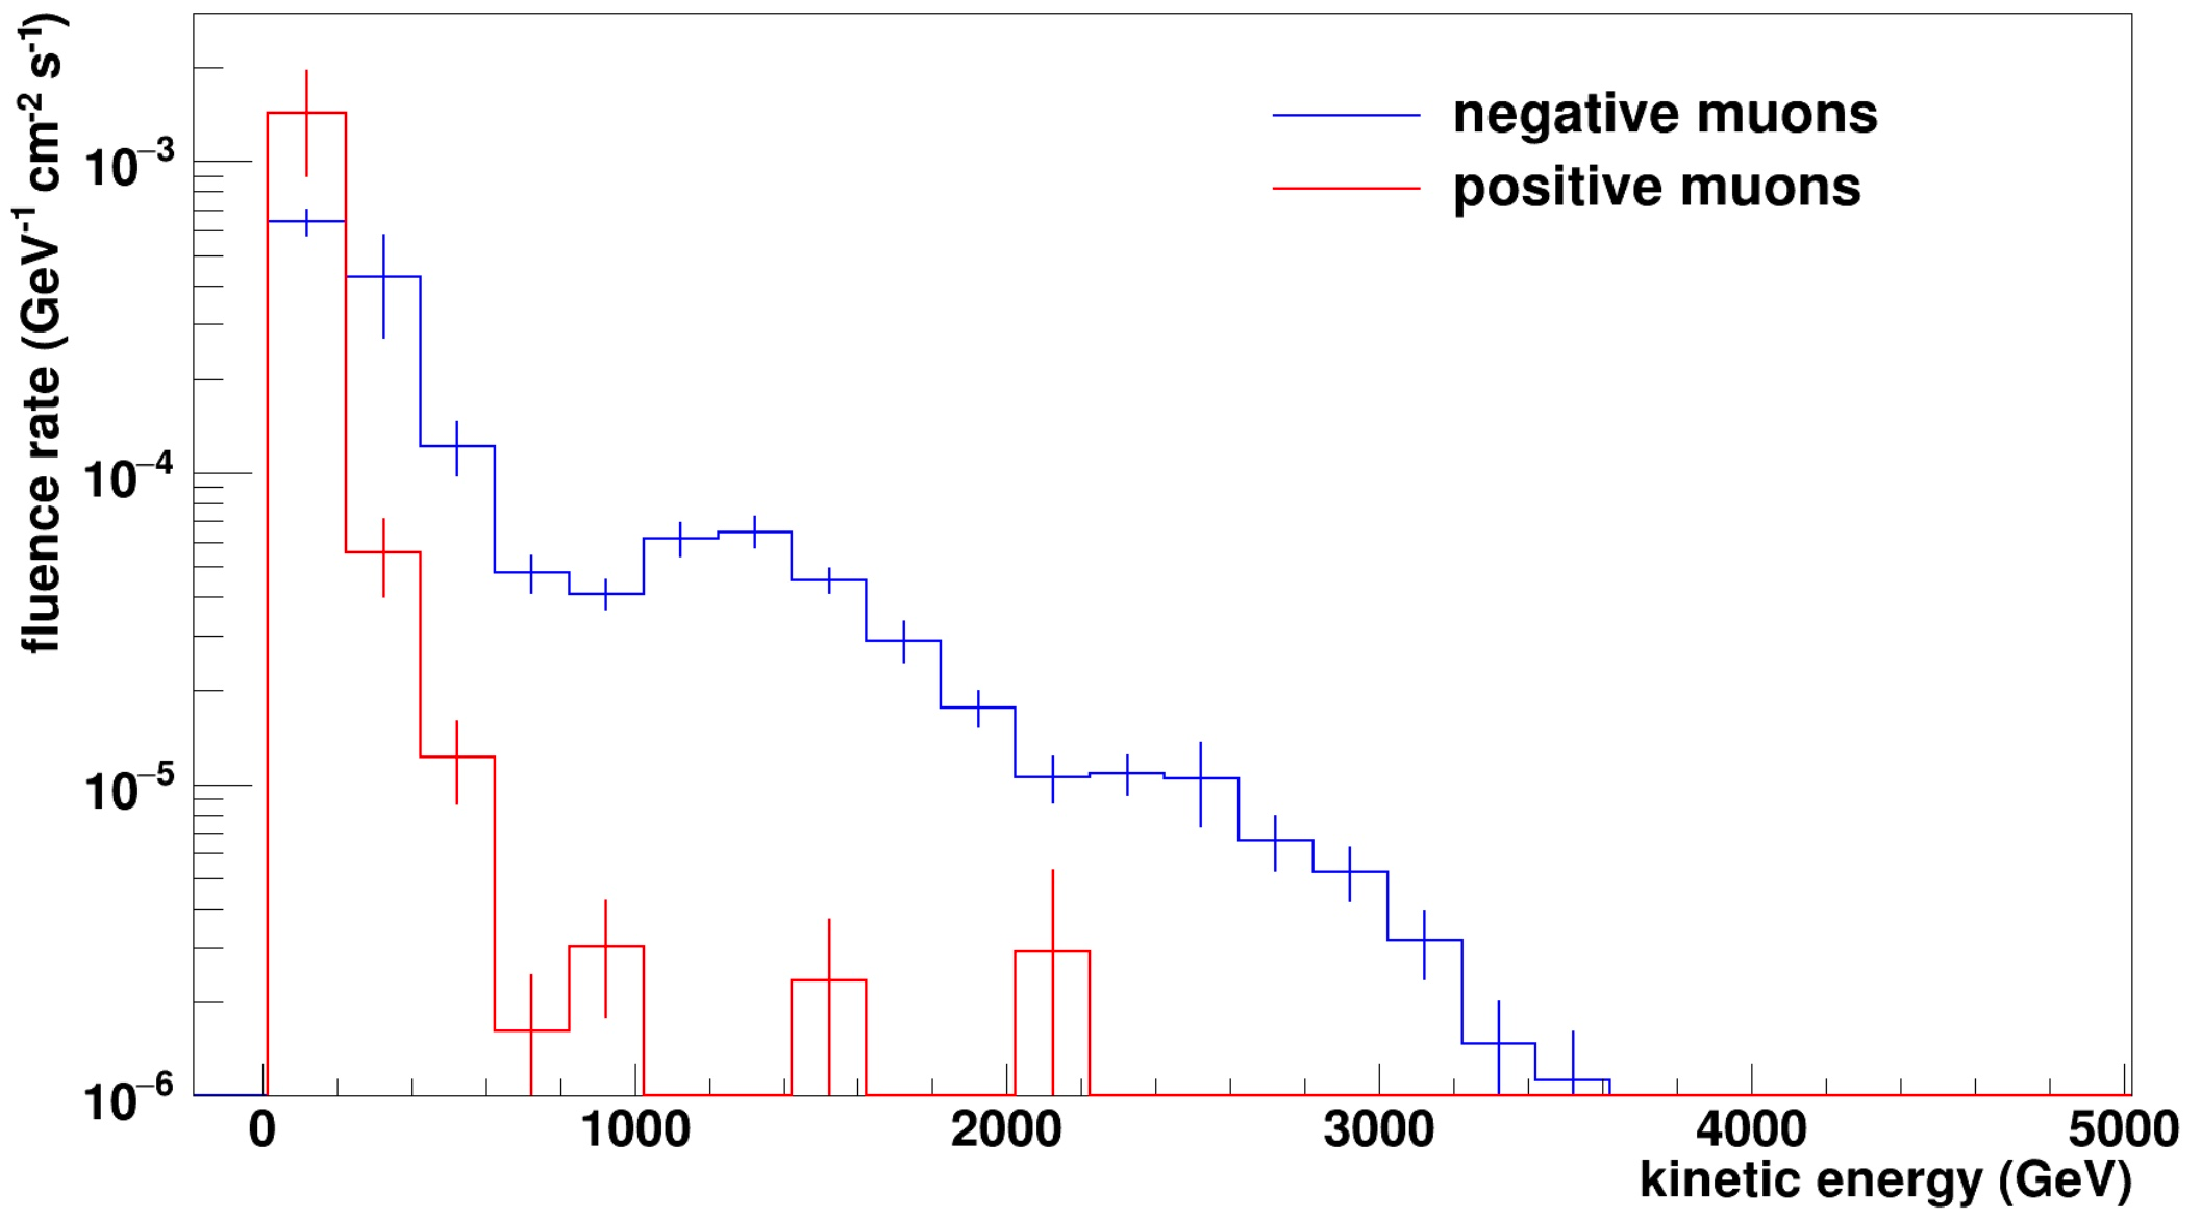
\includegraphics[width=0.8\linewidth]{files/muon_flux}
				\caption{FLUKA simulations estimations of the muon flux as a function of the energy. The flux is given separately for $\mu^+$ (in red) and $\mu^-$ (in blue). The flux is normalised to a luminosity of $2 \times 10^{34}$ cm$^{-2}$ s$^{-1}$}
				\label{im:muon_flux}
			\end{figure}
			
			The flux for $\mu^+$ and $\mu^-$ is very different due to the due to the bending of the magnets from the LHC. For particles above \SI{10}{\giga\electronvolt} the muon traversal rate per surface unit is of the order of \SI{0.4}{\hertz\centi\meter}$^{-2}$. The particles produced by interaction of the neutrinos in the material have not been taken into account as their contribution is several order of magnitude lower. The location of FASER is very strategic as it sits in a region where the muon flux is particularly low with respect to surrounding areas (within \SI{2}{\meter}) as show in \cite{FASER_techprop}.\\

			The copious amount of muons reaching FASER could produce signatures mimicking those of the decay of an LLP in the following ways:  
			\begin{itemize}
    			\item \textbf{Hard Bremsstrahlung:} A high-energy muon can emit a bremsstrahlung photon in the detector material, producing an $e^+e^-$ pair and mimicking an electromagnetic LLP decay such as the one of the dark photon. If the muon was to produce two consecutive photons, highly collimated and not converting in the detector material, this could also lead to a fake di-photon ALP signature. 
    			\item \textbf{Direct Pair Production:} Muons can directly produce $e^+e^-$ pairs via interactions in the detector, also faking a displaced electromagnetic vertex for the dark photon.
    			\item \textbf{Muon Catastrophic Energy Loss:} Rare catastrophic losses can deposit significant energy, appearing as highly energetic showers.
			\end{itemize}
		
			\subsubsection{Neutrino-induced backgrounds}  
			Neutrinos in the forward direction are predominantly produced in the decays of hadrons which can either occur at the IP itself or further down the beam pipe and travel essentially unimpeded to FASER. The neutrino energy spectrum extends from a few GeV up to several TeV as shown in figure \ref{im:neutrino_flux}.
			\begin{figure}[h]
				\centering
				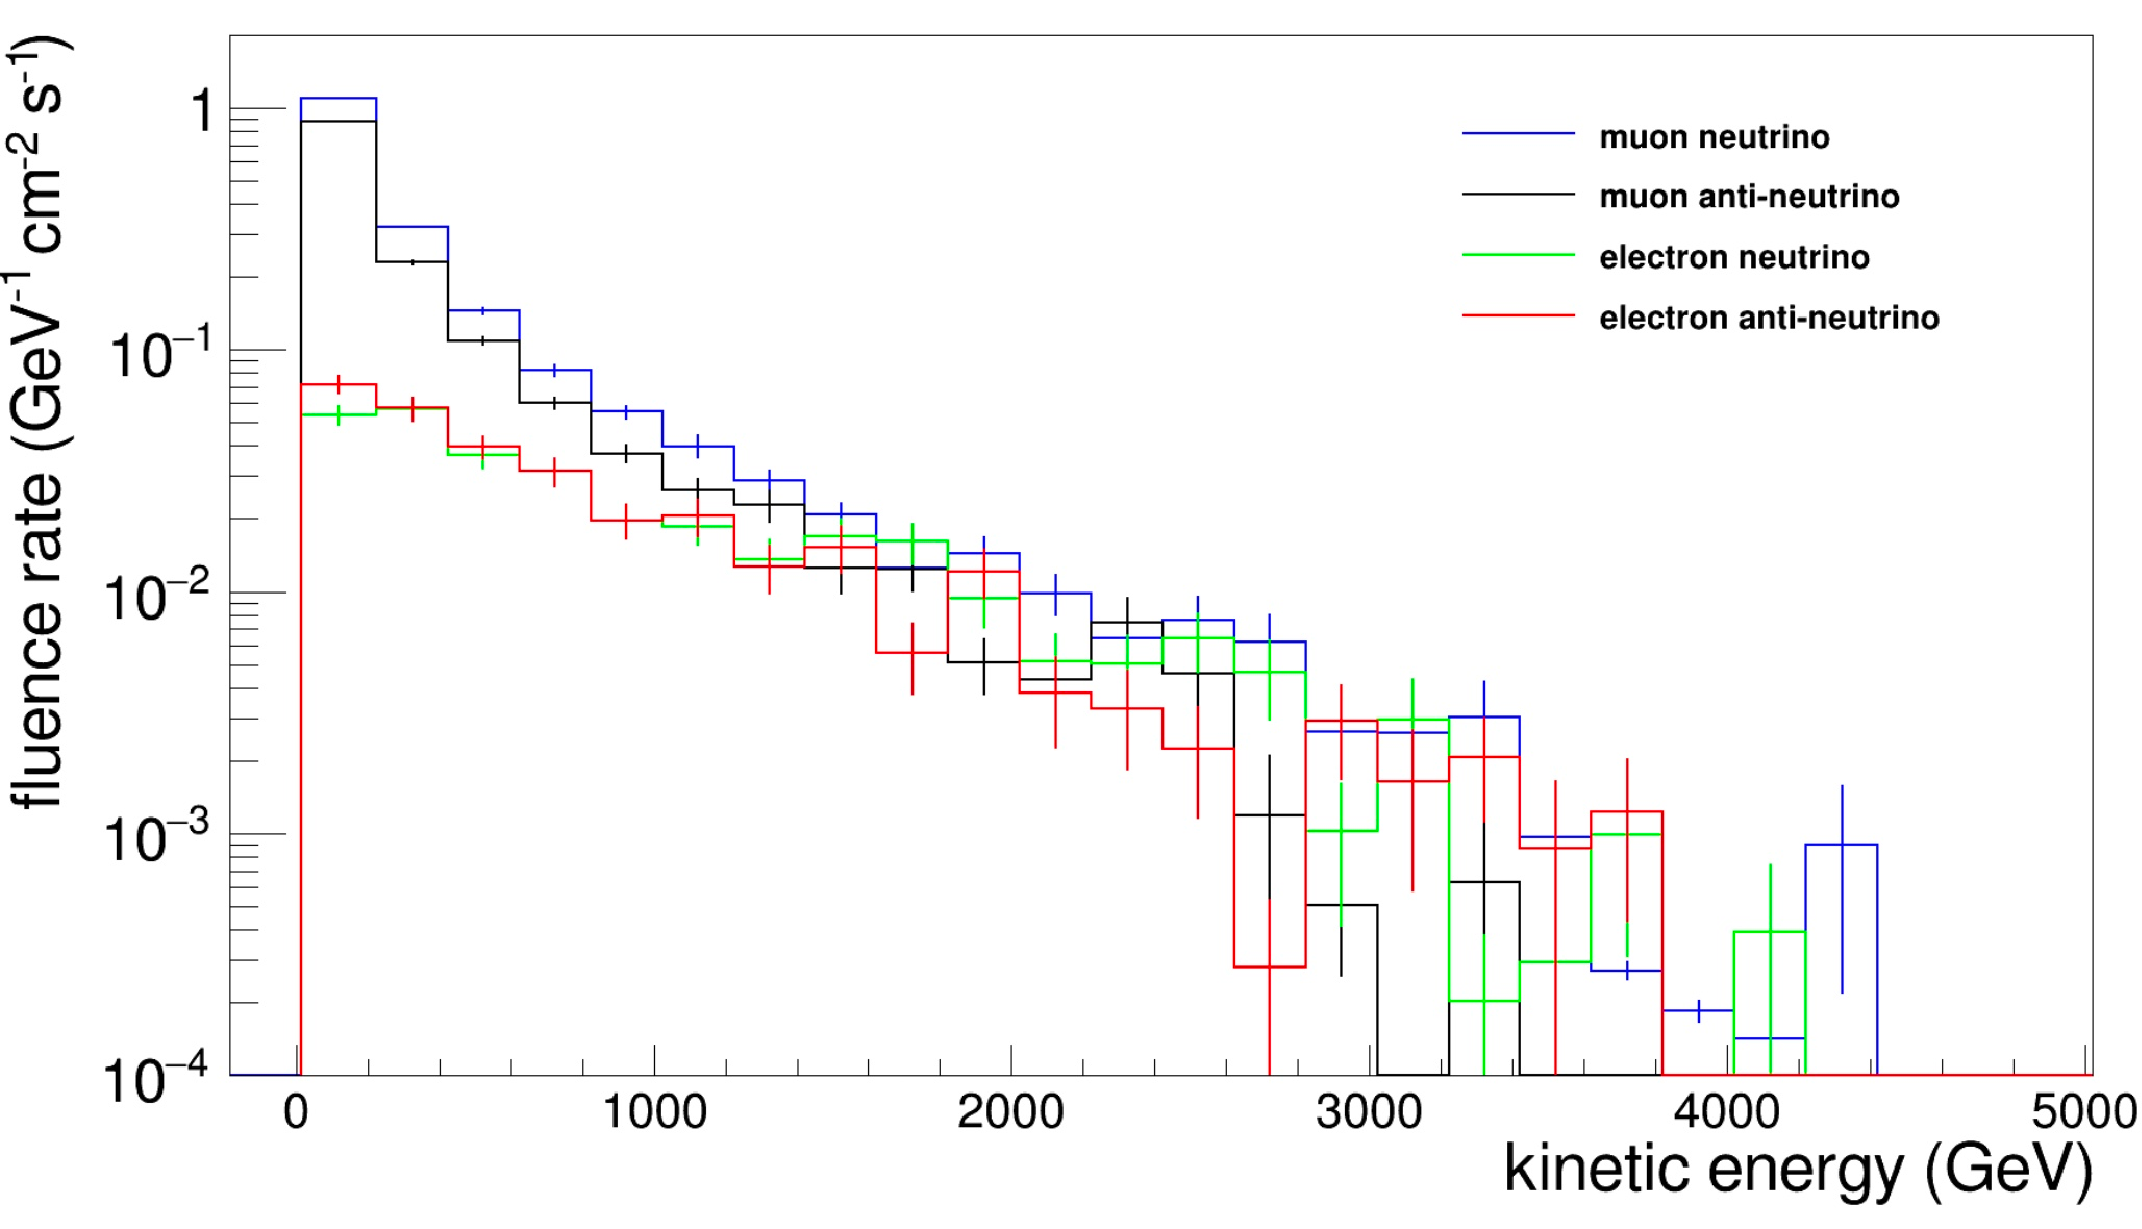
\includegraphics[width=0.8\linewidth]{files/neutrino_flux}
				\caption{FLUKA simulations estimations of the neutrino flux as a function of the energy. The flux is given separately for $\nu_{e}$ (in red) $\nu_{\mu}$ (in blue) $\bar{\nu}_{\mu}$ (in black) and $\nu_{\tau}$ (in green). The flux is normalised to a luminosity of $2 \times 10^{34}$ cm$^{-2}$ s$^{-1}$}
				\label{im:neutrino_flux}
			\end{figure}

			Neutrino CC interactions inside the detector can mimic LLP decays by producing visible final-state charged leptons or hadronic activity emerging from a seemingly empty region. However, neutrino interaction rates are drastically suppressed by their small cross section.
			While irreducible in principle, the neutrino-induced background remains extremely small compared to potential LLP signals.

		\subsubsection{Beam-induced backgrounds}  
		Additional backgrounds could arise from beam-gas interactions (collisions between LHC protons and residual gas molecules) or beam losses in the accelerator infrastructure. GEANT4-based studies including measured vacuum conditions demonstrate that such backgrounds are suppressed by several orders of magnitude relative to the muon flux and are negligible~\cite{FASER_techprop}.


		\subsubsection{Validation with in situ measurements}  
		During Run 2, emulsion-film detectors installed on the beam collision axis in TI12 measured the charged-particle fluence directly. The observed flux of $(1.2-1.9)\times10^4$~cm$^{-2}$~fb$^{-1}$ within \SI{10}{\milli\radian} matches simulation predictions \cite{FASER_techprop}. These measurements confirm the FLUKA modelling of particle fluxes at FASER’s location and validate that no unexpected backgrounds are present. A complementary measurement with a TimePix beam-loss monitoring system shows a correlation between the rate of charged particles and the ATLAS luminosity as expected from the FLUKA simulations. \\
		
		This overview of the different source of background from the SM to LLP decay signatures imposes new constraints on the layout of the detector in order to be able to nicely separate signals from and beyond the Standard Model. 
		
		\subsection{Detector requirements}
		
		In order for FASER to fully exploit its physics program on the hidden sector and neutrino cross section measurements, a specific set or requirements on the layout of the detector are imposed. The distinction from SM induced signatures and pure LLP decay signatures must also guide the design of the detector. An overview of the most relevant requirements on the FASER detector is presented below. 
		
		\subsubsection{Position within TI12 tunnel}
		The FASER detector must be precisely aligned on the ATLAS LoS to within \(\pm10\)\,cm for all beam–crossing angles, in order to maximise both the acceptance of LLP signatures and the energy of neutrinos traversing the active volume. \cite{FASER_Detector}. In order to suppress the large background of high‐energy muons produced at the ATLAS IP, the detector must include a veto system for charged particles entering the detector with an inefficiency smaller than $10^{-9}$ since the expected number of muons entering FASER throughout Run 3 is estimated to me $\mathcal{O}(10^9)$ \cite{FASER_Detector}.
		
		\subsubsection{Energy and Momentum measurements}
		A tracker for high-energy charged particle with good spatial precision is essential in the design of the detector. For a dark photon with mass $m_{A'} =$ \SI{100}{\mega\electronvolt} reaching FASER with a momentum of \SI{2}{\tera\electronvolt}, the expected opening angle of the decay products is $\sim $ \SI{50}{\micro\radian}. A magnet with consequently designed bending power needs to be able to separate the opposite charged tracks of highly boosted LLP decays up to measurable distance by the tracker. The tracker together with the magnet is often referred to as the tracking spectrometer. It is also required to be able to measure the charge of the muons produced in $\nu_{\mu}$ and $\bar{\nu}_{\mu}$ interactions, up to a momentum of several hundreds \SI{100}{\giga\electronvolt}.
		
		To complement the momentum measurement of the spectrometer, an electromagnetic calorimeter is placed downstream. Capacity of measuring TeV‐scale energy deposits with a few‐percent resolution is required to reconstruct e\(^{+}\)e\(^{-}\) or \(\gamma\gamma\) final states from dark‐sector decays such as dark photon or ALPs.
		
		\subsubsection{Large target mass detector for neutrinos}
		Within the tight spatial constraints of the TI12 tunnel, a compact, high‐density neutrino target is needed to collect a sufficient amount of CC interactions. The detector must be able to identify muons, electrons (and distinguish them from gamma rays), and identify short‐lived \(\tau\) and charm decays through a combination of passive material, finely‐segmented active layers, and excellent vertex and angular resolution.  A precision tracker immediately downstream of the emulsion‐based system facilitates the matching of tracks between the passive and active elements, reducing combinatorial ambiguities by $\mathcal{O}(10^{6})$ via a scintillator veto on front‐stack triggers \cite{FASER_Detector}.
		
		
		\subsubsection{Trigger and Data acquisition}
		The trigger and data‐acquisition system must operate robustly at a muon‐induced rate of $\mathcal{O}(650\,\mathrm{Hz})$ for a luminosity of $2\times10^{34}\,\mathrm{cm}^{-2}\mathrm{s}^{-1}$, with minimal dead time to ensure high efficiency for rare events. Finally, FLUKA simulations and 2018 BatMon measurements predict a low‐radiation environment annual doses below $5\times10^{-3}\,\mathrm{Gy}$ and neutron fluence below $5\times10^{7}\,\mathrm{cm}^{-2}$ allowing the use of conventional (non–radiation‐hard) electronics.
 

		\subsection{Original detector layout}
		
		Once the physics program of the FASER detector was defined, a careful study of the typical decay channels of most prominent LLP model, together with possible signals from high energy collider neutrinos shaped its layout. To minimise other SM signals altering the sensitivity of very rare BSM events in FASER, complementary requirements helped defining the detector layout as it will be presented in figure \ref{im:FASER_layout}.
			\begin{figure}[h]
				\centering
				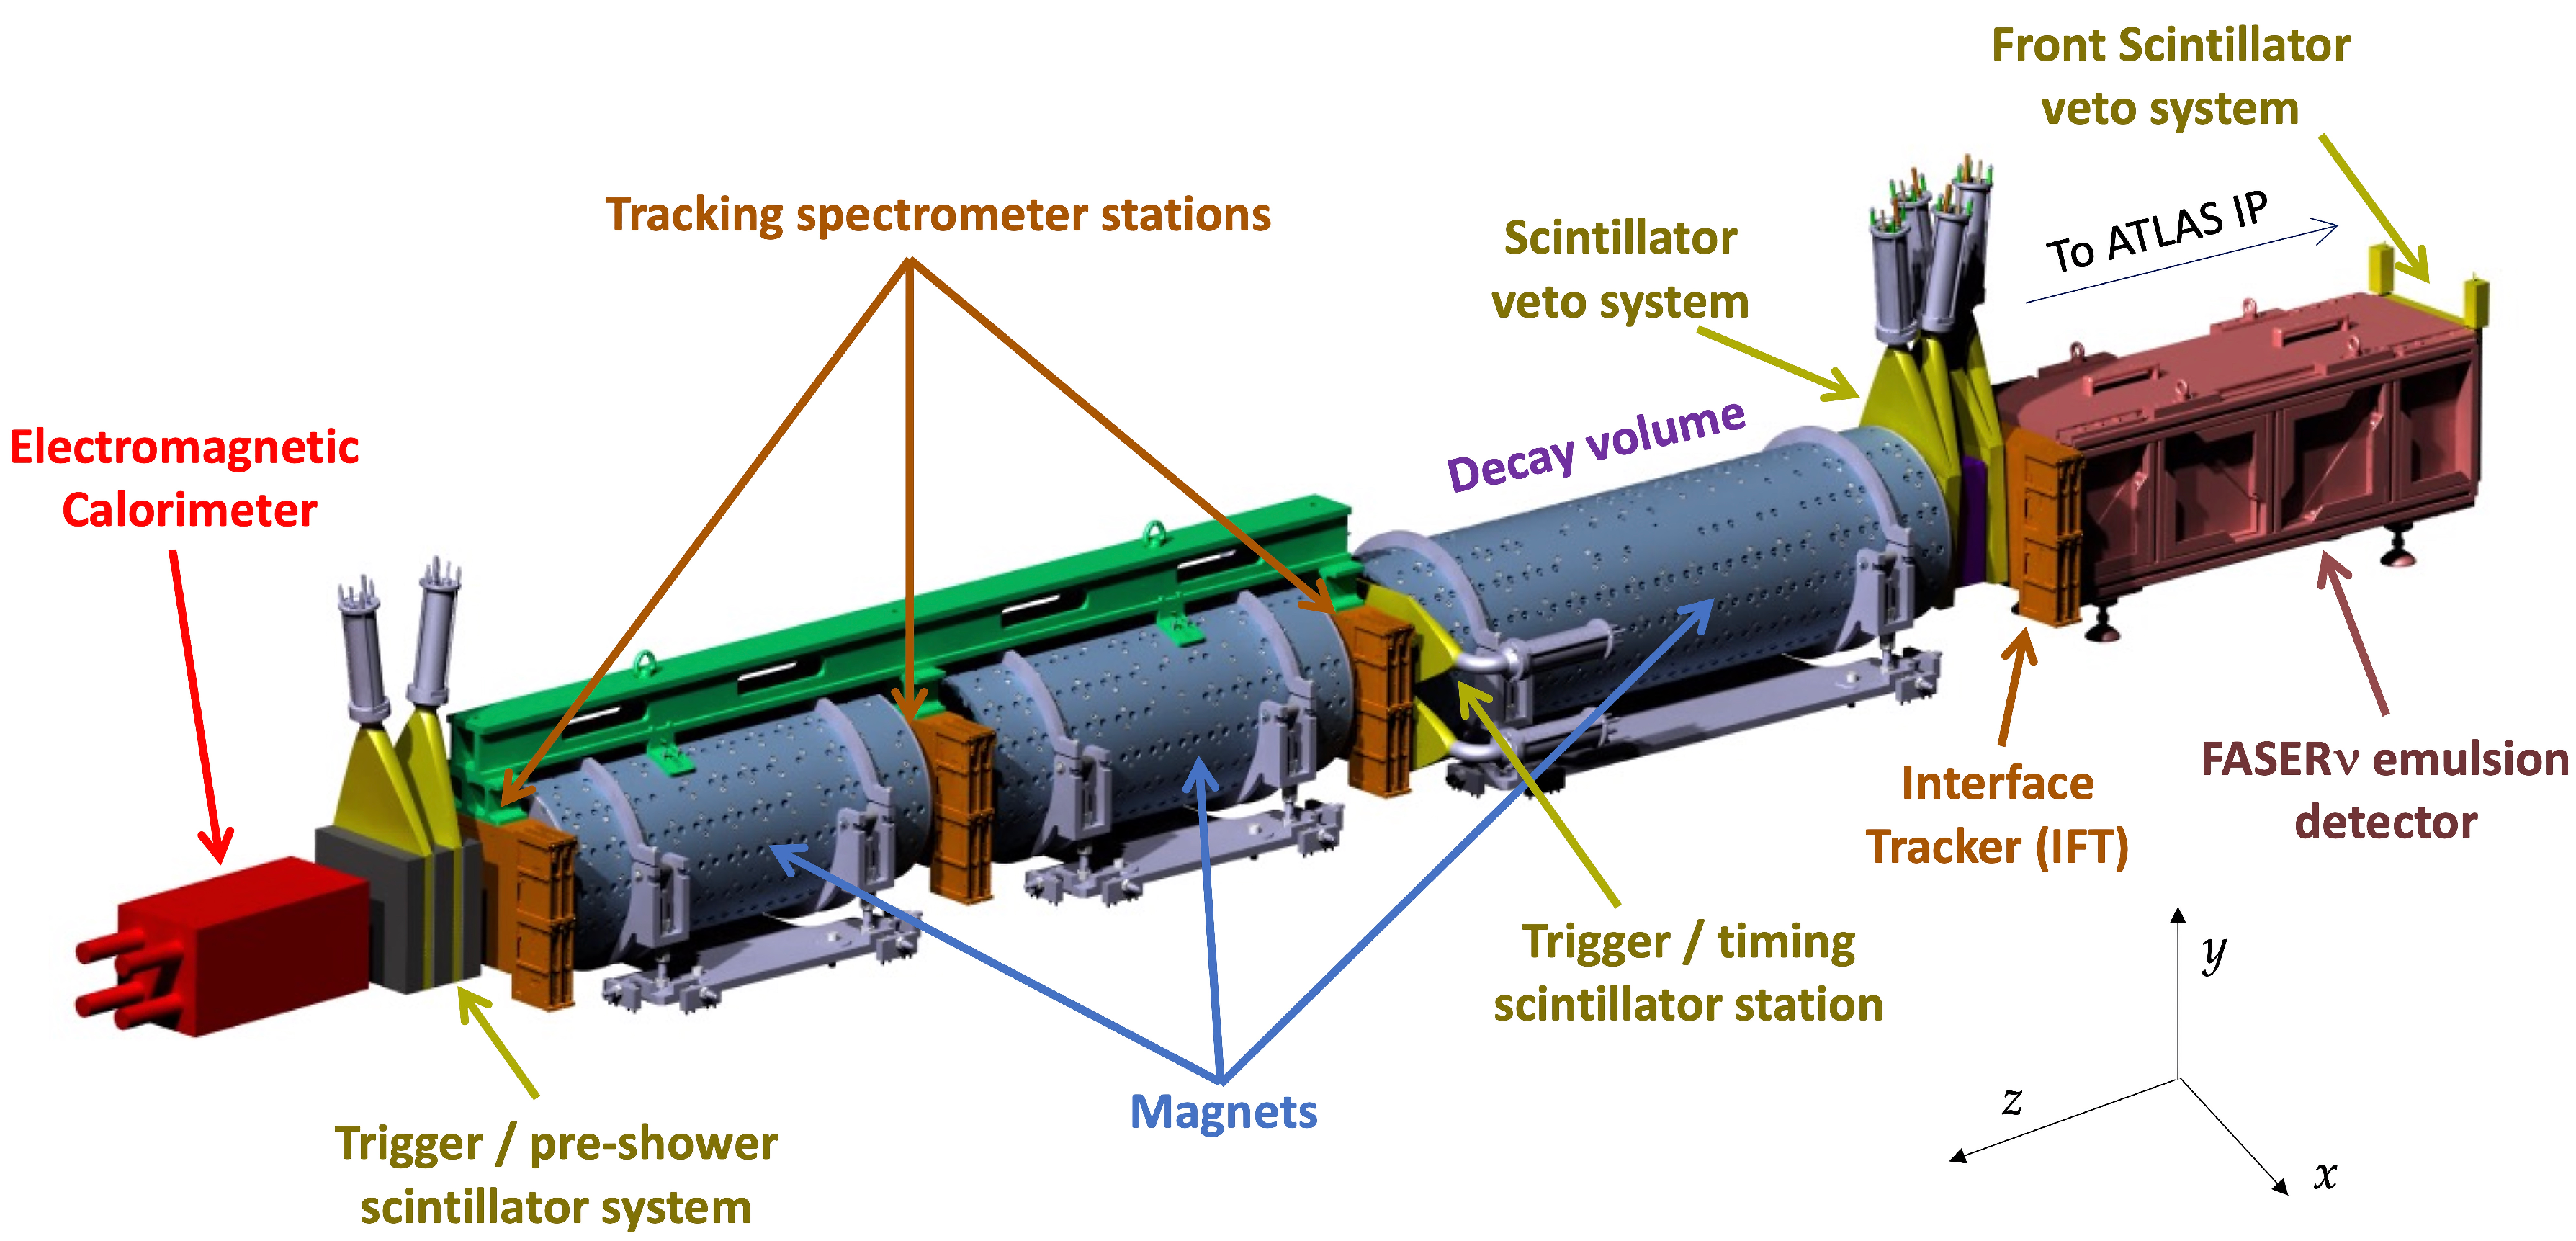
\includegraphics[width=0.9\linewidth]{files/FASER_layout}
				\caption{Layout of the FASER detector with the addition of the FASER$\nu$ detector.}
				\label{im:FASER_layout}
			\end{figure}
			
		Other factors such as short available time for design, construction, commissioning and installation motivated the used of already existing detector components. This helped reducing the cost of the detector while minimising the services and installation works required. The detector can be separated into different modules, each of them having one or more purposes and often acting as a whole, both for event reconstruction and vetoing. 
		
			\subsubsection{The magnet system}
			One of the key elements of the FASER detector is the set of three dipole magnets producing a \SI{0.57}{\tesla} magnetic field inside the decay volume and the tracking spectrometer. Permanent magnets were specifically chosen and designed for the detector, aiming at a reduced amount of services required for operation. The magnets have a \SI{20}{\centi\meter} aperture at the center and their outer radius extends to \SI{43}{\centi\meter}, the first magnet is part of the decay volume and is \SI{1.5}{\meter} long while the other two magnets are part of the tracking spectrometer and are both \SI{1.0}{\meter} long. 
				
			The aim of having magnets is the ability to separate the tracks of charged decay products, mainly the electron-positron pair (or more rare muon anti-muon pair) coming from a Dark Photon decay. The system is also tasked with measuring the charge of muons produced in neutrinos interactions. The magnetic field outside of the magnet should be as small as possible in order not to affect the readout of other detector subcomponents such as PhotoMultiplier Tubes (PMTs). 
		
			\subsubsection{The tracking system}
			The tracking system of the FASER detector can be divided into two separate systems: the Interface Tracker (IFT) and the tracking spectrometer. The IFT is a single tracking station located right after the FASER$\nu$ emulsions detector where as the tracking spectrometer is composed of three tracking stations located at the end of each dipole magnet (see figure \ref{im:FASER_layout}). 
			
			The IFT and tracking spectrometer operate synergistically. The tracking spectrometer is tasked with the reconstruction of the trajectories of charged particles crossing the detector. It provides both a position and momentum measurement and can also identify the charge of muons arising from neutrino interactions. The IFT provides a matching between the tracks reconstructed in the emulsion detector and the tracks registered in the active detectors \cite{FASER_Detector}. A timestamp can be associated to reconstructed tracks in the emulsion detector from neutrino interaction, hence using the tracking system information for muon identification. The information from the rest of the detector can further be used for background rejection and better reconstruction of the neutrino energy \cite{FASER_Detector}. 
			
			The two systems consist of three double-layers of single sided silicon microstrip detectors. Each layer is made of eight silicon strip modules and are spares from the ATLAS experiment's SCT barrel detector \cite{SCT_ATLAS}. Each SCT module cover an area of $6 \times 12$ cm$^2$ and they are arranged in 2 columns made of 4 modules to cover a total active area of $24 \times 24$  cm$^2$, hence covering the full aperture of the magnets. The SCT modules are made of two silicon layers, assembled with a small stereo angle of \SI{40}{\milli\radian} providing a \SI{20}{\micro\meter} resolution in the bending plane and \SI{800}{\micro\meter} otherwise. In terms of performances the tracking spectrometer have a well above 99 $\%$ detection efficiency (per SCT module) and is able to distinguish particles tracks separated by $100-200$ $\mu$m. The IFT is capable of providing a track angular resolution  of \SI{250}{\micro\radian} in the bending plane and \SI{13}{\milli\radian} otherwise.  
			  
			 \subsubsection{The Scintillator and calorimeter systems}
			 The detector is instrumented with four different scintillator stations contributing both to vetoing unwanted background events and triggering. These stations are placed before and after the FASER$\nu$ emulsion detector and on both ends of the tracking spectrometer (see figure \ref{im:FASER_layout}). The electromagnetic calorimeter is placed right after the last scintillator station. Its purpose is to measure the energy of high-energy electrons and photon and also take part in triggering for signals with large energy deposition. 
			 
			 The first two stations are essential in assessing whether or not a charged particles entered the detector. The station in front of the FASER$\nu$ emulsion detector is made of two scintillator counter while the second station is made of four scintillator counters. Each scintillator is read out by a dedicated PMT. The scintillator cover a larger area that the aperture of the magnets, this helps with vetoing charged particles entering FASER with an angle, their inefficiency has to be compatible with the high muon rate expected on their full active area. 
			 
			 The third scintillator station, also known as the timing station is made of two scintillator counters and are each read out by two PMT on each side in the transverse plane. This station detect whether or not charged particles enter the tracking spectrometer and assigns a precise time for triggered events (with a resolution better than \SI{1}{\nano\second}) \cite{FASER_Detector}.
			 
			 The fourth and last scintillator station, also known as the pre-shower station is composed of two scintillator counters, readout by a single PMT. Each scintillator in the station is preceded by a \SI{3}{\milli\meter} thick layer of tungsten and a graphite layer to reduce backsplash from the calorimeter is placed between right after the second scintillator counter. The aim of the pre-shower in this configuration is to help distinguishing between neutrino and photon events in the calorimeter. 
			 
			 Finally, the electromagnetic calorimeter  The station is made of a squared arrangement of four spare modules from the LHCB experiment's outer electromagnetic calorimeter (ECAL) \cite{FASER_Detector}. The sampled design of 66 interleaved layer of lead and plastic scintillator with wavelength shifting fiber driving the collected light to a PMT at the back of each module, offers a total of 25 radiation length and provides an energy measurement with a precision at the percent level in the energy regime needed. It unfortunately offers no transversal position measurement and is unable to distinguish separate two particle tracks. 
			 
			 \subsubsection{The FASER$\nu$ emulsion detector}
			 Initially not in the very first detector layout presented in \cite{FASER_loi, FASER_techprop}, the FASER$\nu$ emulsion detector was added at the very front of the FASER detector to study high energy neutrinos produced in colliders. The detector weights a total of \SI{1.1}{\tonne} and is made of 770 interleaved layers of 1-mm thick tungsten plates for neutrino to interact and emulsion films recording the tracks of charged particles  with excellent position and angular resolution \cite{FASER_Detector}. Oppositely to the rest of the FASER detector, the emulsion detector is passive and readout of the information recorded by the emulsion films requires extraction development and scans of each film before reconstruction of the particle trajectories. 
			 
			 The detector essentially detects neutrinos CC interactions through the identification of the lepton track associated to the vertex. A detailed explanation of how different neutrinos interactions of different flavours can be identified is given in \cite{FASER_Detector}. Since the detector record every charged particle crossing its volume, the track resolution allows for a multiplicity of the order of $\mathcal{O}(10^6)$ per cm$^2$ before it needs to be replaced, which is equivalent to an exposure to $30$-$50$ fb$^{-1}$ of collision data \cite{FASER_Detector}. 
			 
			 \subsubsection{Trigger and Data Acquisition}
			 
			 As previously anticipated, the FASER detector is triggered by any signal in any of the scintillator stations or the calorimeter. The trigger rate essentially comes from muons around the LOS, for the aperture of the magnet, the rate would be \SI{150}{\hertz} but since the scintillator stations were designed with a larger acceptance that the aperture ($40\times 40$ cm$^2$) the expected rate rises to \SI{650}{\hertz}. A schematic and simplified view of the FASER Trigger and Data Acquisition (TDAQ) architecture is given in figure \ref{im:FASER_TDAQ}.
			 \begin{figure}[h]
				\centering
				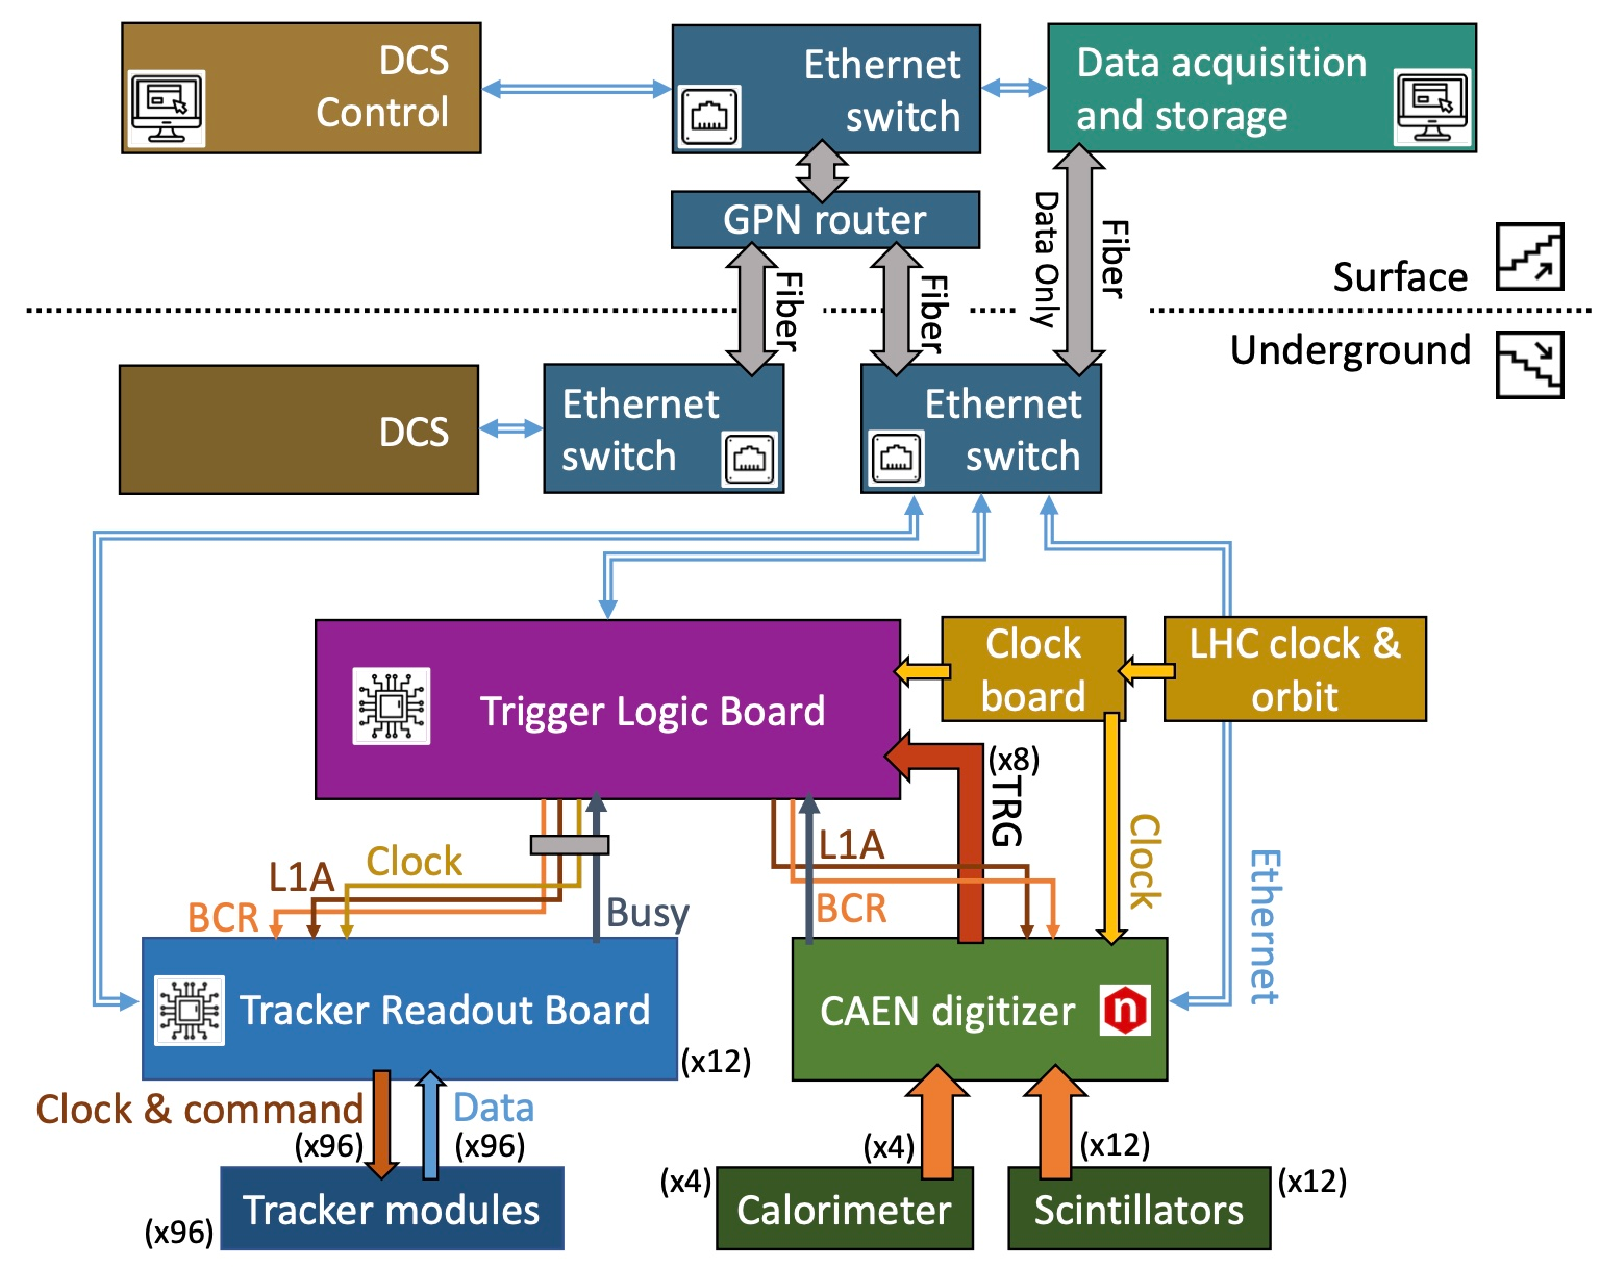
\includegraphics[width=0.8\linewidth]{files/FASER_TDAQ}
				\caption{Schema of the FASER TDAQ architecture. The number in parentheses indicate the number of channels or lines \cite{FASER_Detector}.}
				\label{im:FASER_TDAQ}
			\end{figure}	 
			
			The raw signals from the PMTs of all four calorimeters modules and the tracking stations (for a total of 12 channels) are sent to a commercial digitizer with a pre-defined threshold. The output trigger signal is sent to a custom Field Programmable Gate Array (FPGA)-based Trigger Logic Board (TLB), combining the inputs to form a global trigger, called Level 1 Accept (L1A) trigger. The TLB is able to pre-scale and inhibits certains trigger, it also offers the possibility to do monitoring. Once generated, the L1A signal is sent to the Tracker Readout Boards (TRBs) and the digitizer for initiating the readout of the detector data. A dedicated optical fiber network is in charge of transferring data sent by the readout boards to a software event builder DAQ running on a surface-located server. The TDAQ system's hardware operates at the LHC clock of $\sim$\SI{40}{\mega\hertz}, received and processed via dedicated electronics to correct for jitter and phase shifts throughout running \cite{FASER_Detector}. 
			 
		\subsection{Charged and neutral decay signatures from LLPs}
		The layout fo the FASER detector defined, it is interesting to study the different signatures of the typical LLP decay FASER could observe. Two signatures were previously identified, namely for the dark photon, a decay into a pair of oppositely charged leptons, mostly an $e^+ \hspace{1mm} e^-$ pair and for the ALP a pair of photons. \\ 
		
		The typical signature for a dark photon decay into a lepton pair is presented in figure \ref{im:FASER_OLD_DP_signature}: 
		\begin{figure}[h]
			\centering
			\includegraphics[width=1.0\linewidth]{files/FASER_DP_signature}
			\caption{Typical signature of a dark photon decaying into a pair of oppositely charged leptons ($e^+ \hspace{1mm} e^-$ in this scenario).}
			\label{im:FASER_OLD_DP_signature}
		\end{figure}	
		
		The  decay of a dark photon is hence associated to no signal in the vetoing elements, any signal recorded would indicate a charged particle entering FASER and possibly mimicking an LLP decay signal. Once produced, the oppositely charged lepton pair will be separated by the Lorentz force acting on them, the further down they'll move in the tracking spectrometer, the more they'll separate. It is essential to be able to distinguish the pair of leptons and measure their deviation due to the magnetic field as the precise position measurement offered by the tracking stations in the bending plane allow for a measurement of the momentum of each lepton. Finally, the pair should deposit energy both in the Pre-Shower and the Calorimeter systems, hence providing a measurement of the energy of the lepton pair and hence the dark photon.
		
		The typical signature for an Axion-Like Particle decaying into a photon pair is presented in figure \ref{im:FASER_OLD_ALP_signature}: 
		\begin{figure}[h]
			\centering
			\includegraphics[width=1.0\linewidth]{files/FASER_ALP_signature}
			\caption{Typical signature of an ALP decaying into a pair of photons.}
			\label{im:FASER_OLD_ALP_signature}
		\end{figure}
	
		Similarly, there should be no signal registered in the element of the detector contributing to vetoing. The ALP should decay, leave no presence of its passage through the tracking stations (unless interaction with the tracker material occurs but is very unlikely). A deposit of energy should be recorded in both the Pre-Shower and the Calorimeter systems, signals the presence of at least one photon produced inside the FASER detector. It is important to notice that in this case, the signal for one photon or more than one photo, highly collimated (as suggested if they were originating from the decay of a highly boosted LLP), the FASER detector in its current design wouldn't be bale to distinguish between the two classes of events. For the dark photon the situation is similar if considering only the pre-shower and calorimeter systems but precise spatial information from the tracking stations allows to assess how many charged tracks compose the event. 
	
		The ability to distinguish between a scenario with one photon or more is essential, indeed it was identified previously in \note{section ref to background} that events in which one photon is generated could occur like in muon bremsstrahlung for instance. To fully mimic an ALP decay di-photon event, the muon should perform a double bremsstrahlung with photons begin radiated very close-by, which is very unlikely. Ideally events from muon bremsstrahlung could be vetoed since they will always be accompanied by a signal deposited by the muon in the scintillator stations used for veto. Moreover, with the current design of the pre-shower and calorimeter systems, events in which high energy neutral particles interact would be distinguishable from the event generated by a photon. 
		
		For all of the reasons mentioned above, the possibility to differentiate between the detection of a true decay of LLP into a photonic state and the look-alike events from SM contributions is essential. Upgrading the layout of the detector could unlock the full potential of FASER for a completely novel study of ALPs decay in the di-photon channel bu also extend the physics program to any photonic final state \cite{PreShower_TP}. 
	
	
		
	\clearpage
	\section{Axion Like Particles in FASER}
%		\subsection{Motivation for Axion Like Particles}
		The Axion-Like Particle model with coupling to the photon through the $U(1)$ group of electromagnetic interactions both for the production and decay mechanisms shined light on FASER's sensitivity on the ideal case of a detector with full efficiency \note{section ref here}. In this scenario, the production of ALPs was predominantly associated to the Primakoff Process as explained in \note{section ref}.
		
		Taking one step back, the ALP models originate from the will to bring a solution to the strong CP problem in Quantum ChromoDynamics (QCD). Keeping the discussion at surface level, the QCD axion model is an extension to the SM with the addition of a global chiral $U(1)_{PQ}$ symmetry of the full SM Lagrangian, initially introduced by Peccei and Quinn in 1977 \cite{QCD_axion_PecceiQuinn}. The symmetry is in reality not exact as it would provide an unphysical solution to the strong CP problem. Instead, it has been shown by Peccei and Quinn the $U(1)_{PQ}$ is spontaneously broken, giving rise to a pseudo-Nambu Goldstone boson added to the SM, also knows as the QCD axion. This new particle would contribute to the theoretical prediction of the electric dipole moment of the neutron, reaching an agreement between predictions and measurements. A more complete overview of the strong CP problems and its solutions can be found in \cite{Moretti_MasterThesis}.
		
		The ALP models emerges as a generalisation to the QCD axion solution to the strong CP problem. More recent studies have been focusing on model involving light (with respect to the electroweak scale) pseudoscalar particles, weakly coupled to the SM and appearing in the spontaneous breaking of a global symmetry \cite{ALPs_general}. Previously, only the model with coupling to the photon was considered, but there is no a priori reason why the ALP could not also couple the gluons through the $SU(3)_{QCD}$ group and to weak interactions gauge boson of $SU(2)_L$ group \cite{Moretti_MasterThesis}. Focusing on the second extension, the simplest model in which an ALP (labeled $a$) couples to vector bosons through the dimension-5 operator suggested by the associated Peccei-Quinn symmetry would have additional interaction terms to the Lagrangian such that: 
		\begin{equation}
			\mathcal{L} = -\frac{1}{4} g_{aBB} a B_{\mu\nu} \tilde{B}^{\mu\nu} - \frac{1}{4} g_{aWW} a W_{\mu\nu}^a \tilde{W}^{a,\mu\nu}
		\end{equation} 
		
		In the equation above, the field strength associated to the $U(1)_Y$ group and the $SU(2)_L$ group were respectively labeled as $B_-{\mu \nu}$ and $W_{\mu\nu}^a$ and their coupling to the ALP field were denoted respectively as $g_{aBB}$ and $g_{aWW}$. After ElectroWeak Symmetry Breaking (EWSB), the couplings introduced allow the ALP field to couple to photons and the three gauge bosons responsible for charged and neutral currents in weak interactions. 
		
		Most of the time, only the coupling to photons and gluons are taken into considerations since for low energy regimes (below the electroweak scale), these processes predominantly contribute to the ALP production rates. The coupling to the electroweak gauge bosons is in fact suppressed for energies such that $E < M_{W}$ resulting in very few ALPS produced via this channel \cite{ALPs_general}. Interestingly, the particles produced in the very forward regions of ATLAS in the direction of FASER reach TeV-scale energies, which is well beyond the electroweak scale.    
		
		\subsection{Production from rare meson decays}
		One of the LLP production mechanisms previously described takes advantage of the large hadrons flux in the forward direction, taking its root into rare decay of mesons \note{section ref}. This production channels relies on a processus know as Flavour Changing Neutral Current, in which a down-type quark becomes an up-type quark by emitting a negatively charge boson which itself radiates an ALP. The up-type quark and the charged boson then interacts again, leading to another change in flavour to a down-type quark. Such processes are highly suppressed in the SM by the GIM mechanism \cite{GIM_mechanism} and offers a striking signature for the production channel of the ALP with interesting prospects for discovery. 
		
		In FASER, the ALP can be produced through rare decays of B mesons such as $B \rightarrow K a$ and Kaon such as $K^\pm \rightarrow \pi^\pm a$ or $K_L \rightarrow \pi^0 a$ predominantly. The simulated spectra in the momentum-angle plane for the relevant mesons from the ATLAS IP is given in figure \ref{im:meson_spectra_MC}.
		\begin{figure}[h]
			\centering
			
\includegraphics[width=1.0\linewidth]{files/meson_spectra_MC}
			\caption{Spectrum of in the momentum an angle with respect to beam axis plane for $K_L^0$ mesons (left), $K^\pm$ meson (center) and $B$ mesons (right). The cross section is given per bin in picobarn. A vertical dashed line shows FASER's angular acceptance. The value quoted in the top right corner of each figure gives effective cross section (within FASER's acceptance) and the total cross section.}
			\label{im:meson_spectra_MC}
		\end{figure}
		
		In the context of this discussion, a specific ALP Effective Field Theory (EFT) in its simplest form with only coupling to the $SU(2)_W$ group gauge bosons would lead to a Lagrangian of the form of \cite{Moretti_MasterThesis}:
		\begin{equation}
			\mathcal{L}_{EFT} = \left( \partial_\mu a\right)^2 - \frac{1}{2} M_a^2 a^2 - \frac{g_{aWW}}{4} a W^a_{\mu \nu} \tilde{W}^{a \mu \nu}
		\end{equation} 
		where $a$ is the ALP field, $M_a$ its mass, $W^a_{\mu \nu}$ and $g_{aWW}$ respectively the field strength tensor for $SU(2)_W$ and the coupling of the group's gauge bosons to the ALP field. After EWSB, the coupling gives rises to vertices such as $a \rightarrow W^+ W^-$, $a \rightarrow Z Z$, $a \rightarrow \gamma Z$ and $a \rightarrow \gamma \gamma$ in ratios given by the weak mixing angle. It can be shown that contribution in the Lagrangian to the amplitude of the ALP production through FCNC from a down-type quark takes the form: 
		\begin{equation}
			\mathcal{L}_{d_i \rightarrow d_j} \supset - g_{a d_i d_j} \left( \partial_\mu a \right) \bar{d}_j \gamma^\mu \mathcal{P}_L d_i + h.c.
		\end{equation} 
		where $d_i$ and $d_j$ are respectively the quark fields in the initial and final state and the index $i$ and $j$ can take any value in the flavours of down-type quarks. The indirect coupling of the ALP field to down-type quarks is given by: 
		\begin{equation}
			g_{a d_i d_j} = \frac{2\sqrt{2}G_F M_W^2 g_{aWW}}{16 \pi^2} \sum_{\alpha \in \{u,c,t\}}V_{\alpha i} V^*_{\alpha j} f(\frac{M_{\alpha}^2}{M_{W}^2}) \hspace{5mm} \text{with} \hspace{5mm} f(x) = \frac{x \left( 1+x(log(x)-1) \right)}{(1-x)^2}
		\end{equation}
		where $G_F$ is the Fermi constant, $g_{aWW}$ the ALP coupling to $W^\pm$ gauge bosons and $V_{ab}$ the relevant entries of the Cabibbo-Kobayashi-Maskawa (CKM) matrix \cite{CKM}. In ALP production the terms mediating the FCNC is $g_{a d_i d_j}$. \\
		
		For the leading production processes from mesons in FASER, the Feynman diagrams for the rare decays through FCNC are given in figure \ref{im:meson_decay_FCNC}. In the case of $B$ mesons, the $b$ quark is responsible for the FCNC whereas as for the Kaons, the $s$ quark is the one involved. For the $B$ meson, there exists an alternative process in which it decays into a Kaon excited state $K^*$ but the diagram is very similar. 
		\clearpage
		\begin{figure}[h]
			\centering
			\includegraphics[width=1.0\linewidth]{files/meson_decay_FCNC}
			\caption{Decay through FCNC for leading contributions to ALP production: $B \rightarrow K a$ (left), $K^+ \rightarrow \pi^+ a$ (center) and $K_L \rightarrow \pi^0 a$ (right).}
			\label{im:meson_decay_FCNC}
		\end{figure}
		
		For each diagram, it can be shown that the decay width are given by the following expressions such as \cite{ALPs_general}: 
		\begin{equation}
			\begin{split}
				&\Gamma(B^\pm \rightarrow K^\pm a) = \frac{M_{B^\pm}^3}{64 \pi} \left| g_{abs} \right|^2 \left( 1- \frac{M_{K^\pm}^2}{M_{B^\pm}^2} \right)^2 f_0^2(M_a^2) \lambda^{1/2}(m_{B^\pm}, m_{K^\pm}, m_a) \\
				&\Gamma(B^\pm \rightarrow K^{*\pm} a) = \frac{M_{B^\pm}^3}{64 \pi} \left| g_{abs} \right|^2 A_0^2(M_a^2) \lambda^{1/2}(m_{B^\pm}, m_{K^{*\pm}},m_a) \\
				&\Gamma(K^\pm \rightarrow \pi^\pm a) = \frac{M_{K^\pm}^3}{64 \pi} \left| g_{asd} \right|^2 \left( 1- \frac{M_{\pi^\pm}^2}{M_{K^{\pm}}^2} \right)^2 \lambda^{1/2}(m_{K^\pm}, m_{\pi^\pm}, m_a) \\
				&\Gamma(K_L \rightarrow \pi^0 a) = \frac{M_{K_L}^3}{64 \pi} \text{Im}\left( g_{asd} \right)^2 \left( 1- \frac{M_{\pi^0}^2}{M_{K_L}^2} \right)^2 \lambda^{1/2}(m_{K_L}, m_{\pi^0}, m_a)
			\end{split}
		\end{equation}
		
		For the $B$ mesons decays, the contribution of hadronic form factors given by $f_0(q)$ and $A_0(q)$ are defined in \cite{ALPs_general}. The space phase factor $\lambda$ were also included and can be generally expressed as $\lambda(m_1, m_2, m_3) = \left[ 1- {(m_2 + m_3)^2}/{m_1^2} \right] \cdot \left[  1- {(m_2 - m_3)^2}/{m_1^2} \right]$. One can also write from the above decay rates the branching ratios, essential to compute production rates of ALPs from such processes as \cite{ALPs_general}:
		\begin{equation}
			\begin{split}
				& \mathcal{B}(B^\pm \rightarrow K^\pm a) \simeq 2\cdot 10^4 \times g_{aWW}^2 f_0^2(M_a^2) \lambda^{1/2}(m_{B^\pm}, m_{K^\pm}, m_a) \\
				& \mathcal{B}(B^\pm \rightarrow K^{*\pm} a) \simeq 2 \cdot 10^4 \times g_{aWW}^2 A_0^2(M_a^2) \lambda^{1/2}(m_{B^\pm}, m_{K^{*\pm}},m_a) \\
				& \mathcal{B}(K^\pm \rightarrow \pi^\pm a) = 10.5 \times g_{aWW}^2 \lambda^{1/2}(m_{K^\pm}, m_{\pi^\pm}, m_a) \\
				&\mathcal{B}(K_L \rightarrow \pi^0 a) = 4.5 \times g_{aWW}^2 \lambda^{1/2}(m_{K_L}, m_{\pi^0}, m_a)
			\end{split}
			\label{eq:BR_ALP}
		\end{equation}  
		
		Once the ALPs are produced, they can travel until FASER and since they are usually light, decay into a di-photon pair as the decay channel with heavier gauge bosons would be kinematically forbidden. In order to get an estimation of the number of ALP events expected in FASER, a Monte Carlo (MC) simulation can be performed, taking as input the simulated meson spectrums as in \ref{im:meson_spectra_MC}, make them decay through rare FCNC processes to generate ALPs and hence study the decay of ALPs reaching FASER and the characteristics of the photon pair produced in the final state. This study was performed in \cite{Moretti_MasterThesis} in order to highlight the new prospects of this ALP model and motivate, as anticipated, the need for a modification of the original FASER detector layout.     
		
		The studies were performed with the scope of estimating the number of di-photons events for a specific integrated luminosity of $\mathcal{L}_{int}$. During the simulation, the mass of the ALP $m_a$ and the coupling to electroweak gauge bosons $g_{aWW}$ were free parameters in order to be able to produce a sensitivity reach plot as the one already presented in \ref{im:ALP_photon_prod}. The differential numbers of produced ALPs from any of the meson spectrums can be computed as follows: 
		\begin{equation}
			\frac{dN_{\text{ALP}}}{dp~d\theta} =  \frac{d\sigma_{\text{pp $\rightarrow$ meson}}}{dp~d\theta} \cdot \mathcal{P}_{\text{decay}} \cdot \mathcal{B}(\text{meson} \rightarrow a~X) \cdot \mathcal{L}_{\text{int}}
		\end{equation}
		with the branching ratios given in equation \ref{eq:BR_ALP}, $\mathcal{P}_{\text{decay}}$ the probability that the meson decays and $d\sigma/dpd\theta$ the differential cross section for meson production from proton-proton interaction in the ATLAS IP. This completes the discussion on the production of ALPs from FCNC reaching FASER. It is then interesting so look at their decay into a photon pair, in particular into the characteristics of the di-photon events.  
		
		\subsection{Decay into di-photons}
		For FASER to be sensitive to ALP, they are required to reach FASER and decay within the available volume with is here composed of both the decay volume and the tracking spectrometer ( see figure \ref{im:FASER_layout}). The number of di-photon signals reaching the location were the original pre-shower station is can then be expressed as: 
		\begin{equation}
			N_{\gamma\gamma} = \int \frac{dN_{\text{ALP}}}{dp~d\theta} \cdot \mathcal{P}(p, \theta) \cdot \mathcal{B}(a \rightarrow \gamma~\gamma) \cdot dpd\theta
		\end{equation}
		where the geometrical acceptance was previously defined in \note{section or eq ref} and in this case the branching ratio of the ALP decay into a photon pair is essentially equal to unity. The definition of decay length of the ALP is required in the expression for the probability to decay within the decay volume geometric acceptance and can be expressed as a function of the coupling $g_{aWW}$ using equation \ref{eq:ALP_decay_length} and recalling that the photon coupling $g{a\gamma\gamma}$ can be expressed as: 
		\begin{equation}
			g_{a\gamma\gamma} = \sin(\theta_W)^2 g_{aWW} 
		\end{equation}  
		where the $\theta_W$ is nothing more than Weinberg's angle for quark mixing such that $\sin{\theta_W} \simeq 0.22$ \cite{Weinberg}. 
		
		An estimation of the separation of the two photons is essential for defining the requirements for a detector possibly able to detect the two photons produced in ALP decays. In the center of mass frame of the ALP, the photons are emitted back to back. In order to find the spatial separation between the photons, it is essential to boost their momentum coordinates in the laboratory reference frame. If we label this this angle for each photon by $\theta^*_1$ and $\theta^*_2$, the distance between the photon produced at a position $z_{\text{decay}}$ in a decay volume of length $L$ is given by: 
		\begin{equation}
			\delta_{\gamma\gamma} = {\left( \tan(\theta^*_1) + \tan(\theta^*_2)\right)} \cdot (L-z_{\text{decay}})
		\end{equation}
		
		Both the mass of the ALP $m_a$ and its coupling $g_{aWW}$ have an effect on the topology of the di-photon events. In order to proceed further in the discussion it is unavoidable to specify values for the two free parameters of the model. During the studies performed in \cite{Moretti_MasterThesis}, a large amount of models were probed with mass in the $[0.1-2]$ GeV range and couplings in the $[5\cdot 10^{-7} - 8 \cdot 10^{-4}]$ GeV$^{-1}$ range. A selection of three benchmark models with $\left[m_a, g_{aWW}\right]$ values of $\left[0.165, 1.8\cdot 10^{-4}\right]$, $\left[0.208, 1.0\cdot 10^{-4}\right]$ and $\left[0.32, 3.2\cdot 10^{-5}\right]$ where selected. \\
		
		The spatial distribution in the transverse plane at the position of the original pre-shower is completely uniform for all three models. The distribution of the decay position of the ALP in the direction of the particles entering FASER is also completely flat for all three models. Although, it was shown that the energy of the ALP varies from one model to the other, heavier and more weakly coupled ALPs have a lower most probable energy when decaying inside FASER than the lower mass and higher coupling models. \\
		
		Because of the randomness of the decay angles of the photons with respect to the direction of the momentum of the ALP, the photons energies vary in a wide range. The photon energies distribution is given for the three benchmark models and two additional models with higher masses and smaller couplings in figure \ref{im:ALP_photon_energy}. 
		\begin{figure}[h]
			\centering
			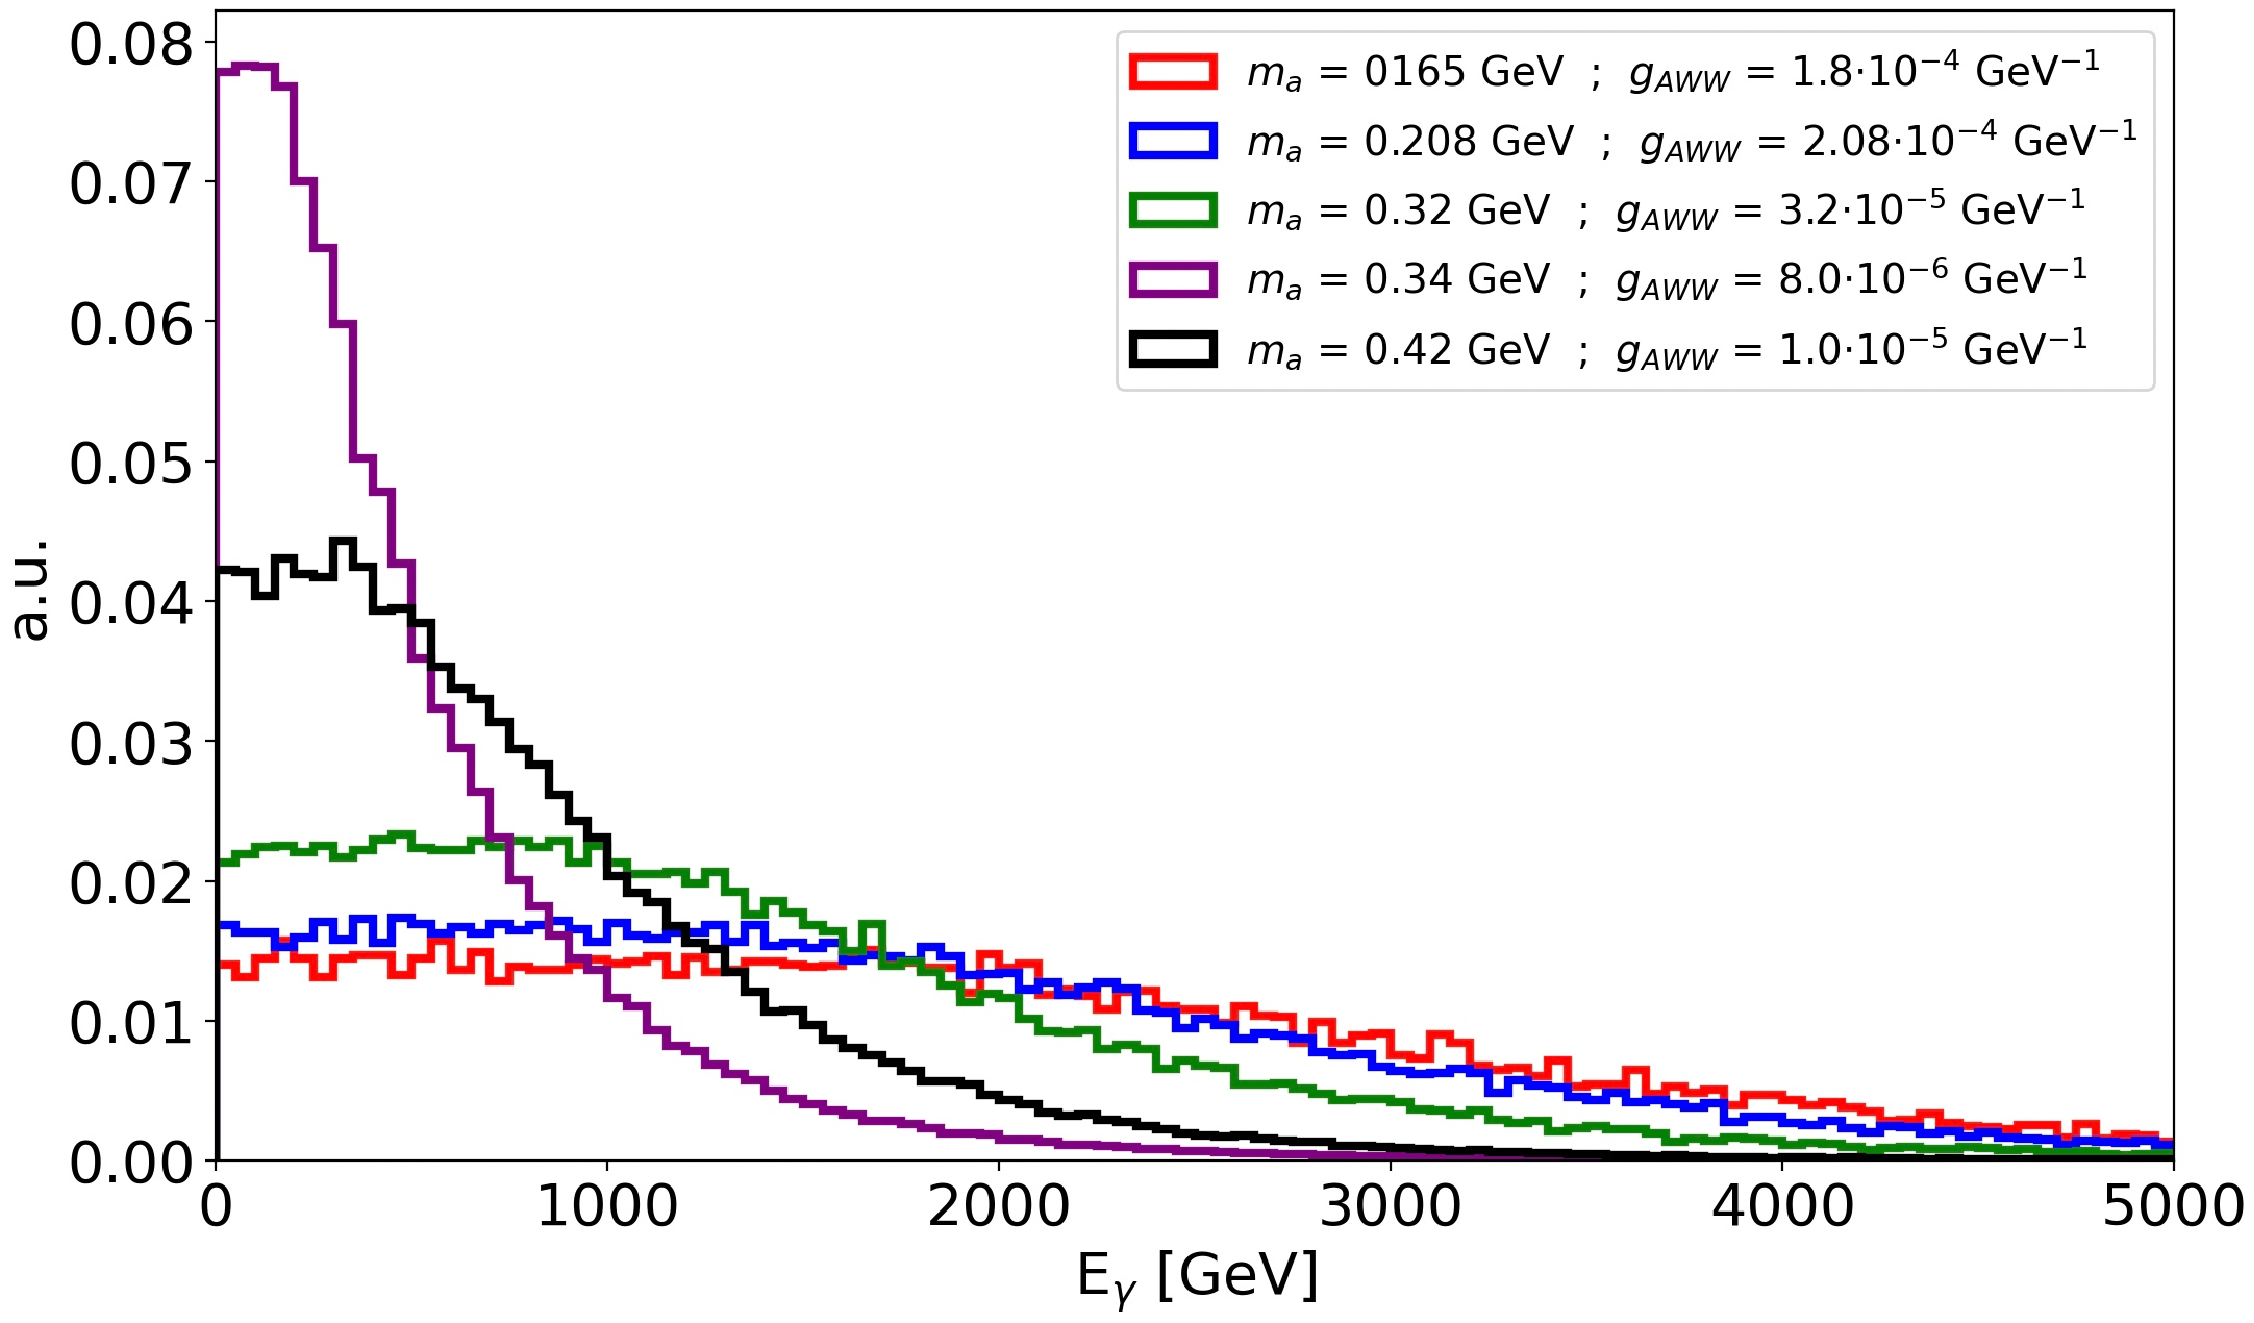
\includegraphics[width=0.8\linewidth]{files/ALP_photon_energy}
			\caption{Energy distribution of the photon emerging from ALP decays for different combination of ALP mass $m_a$ and coupling $g_{aWW}$.}
			\label{im:ALP_photon_energy}
		\end{figure}
		
		It is also interesting to better under the topology of the di-photon production to look at the distribution of number of events in the plane defined by the energy of the two photons separately. This was performed in the studies carried out in \cite{Moretti_MasterThesis} and the results is presented in figure \ref{im:ALP_E1E2_distribution}.
		\begin{figure}[h]
			\centering
			
\includegraphics[width=1.0\linewidth]{files/ALP_E1E2_energy}
			\caption{Energy distribution of the photon emerging from ALP decays for different combination of ALP mass $m_a$ and coupling $g_{aWW}$. The number of events in the top right corner of every figure is given for an integrated luminosity of 90 fb$^{-1}$.}
			\label{im:ALP_E1E2_distribution}
		\end{figure}
		
		As expected the energies of the photon are fully correlated. The distribution show that their exist both events with very similar energies for the photon than events in which the two energies are considerably different. The energies of the two photons depends on the decay angle in the center of mass frame of the ALP, once boosted one of the photon can be very soft while the second one carries most of the momentum of the ALP. To complete the study of ALP production rate, a sensitivity reach plot given in figure \ref{im:reach_plot_ideal} was produced in the mass and coupling. As in the sensitivity reach presented in figure \ref{im:ALP_photon_prod}, an ideal detector with full efficiency and no background events was assumed. Two different reach are presented for different integrated luminosity corresponding to LHC Run3 and HL-LHC.
% TODO CH2: change the scale of the axis and title to match the ones that are bigger in the plots below. 
		\begin{figure}[h]
			\centering
			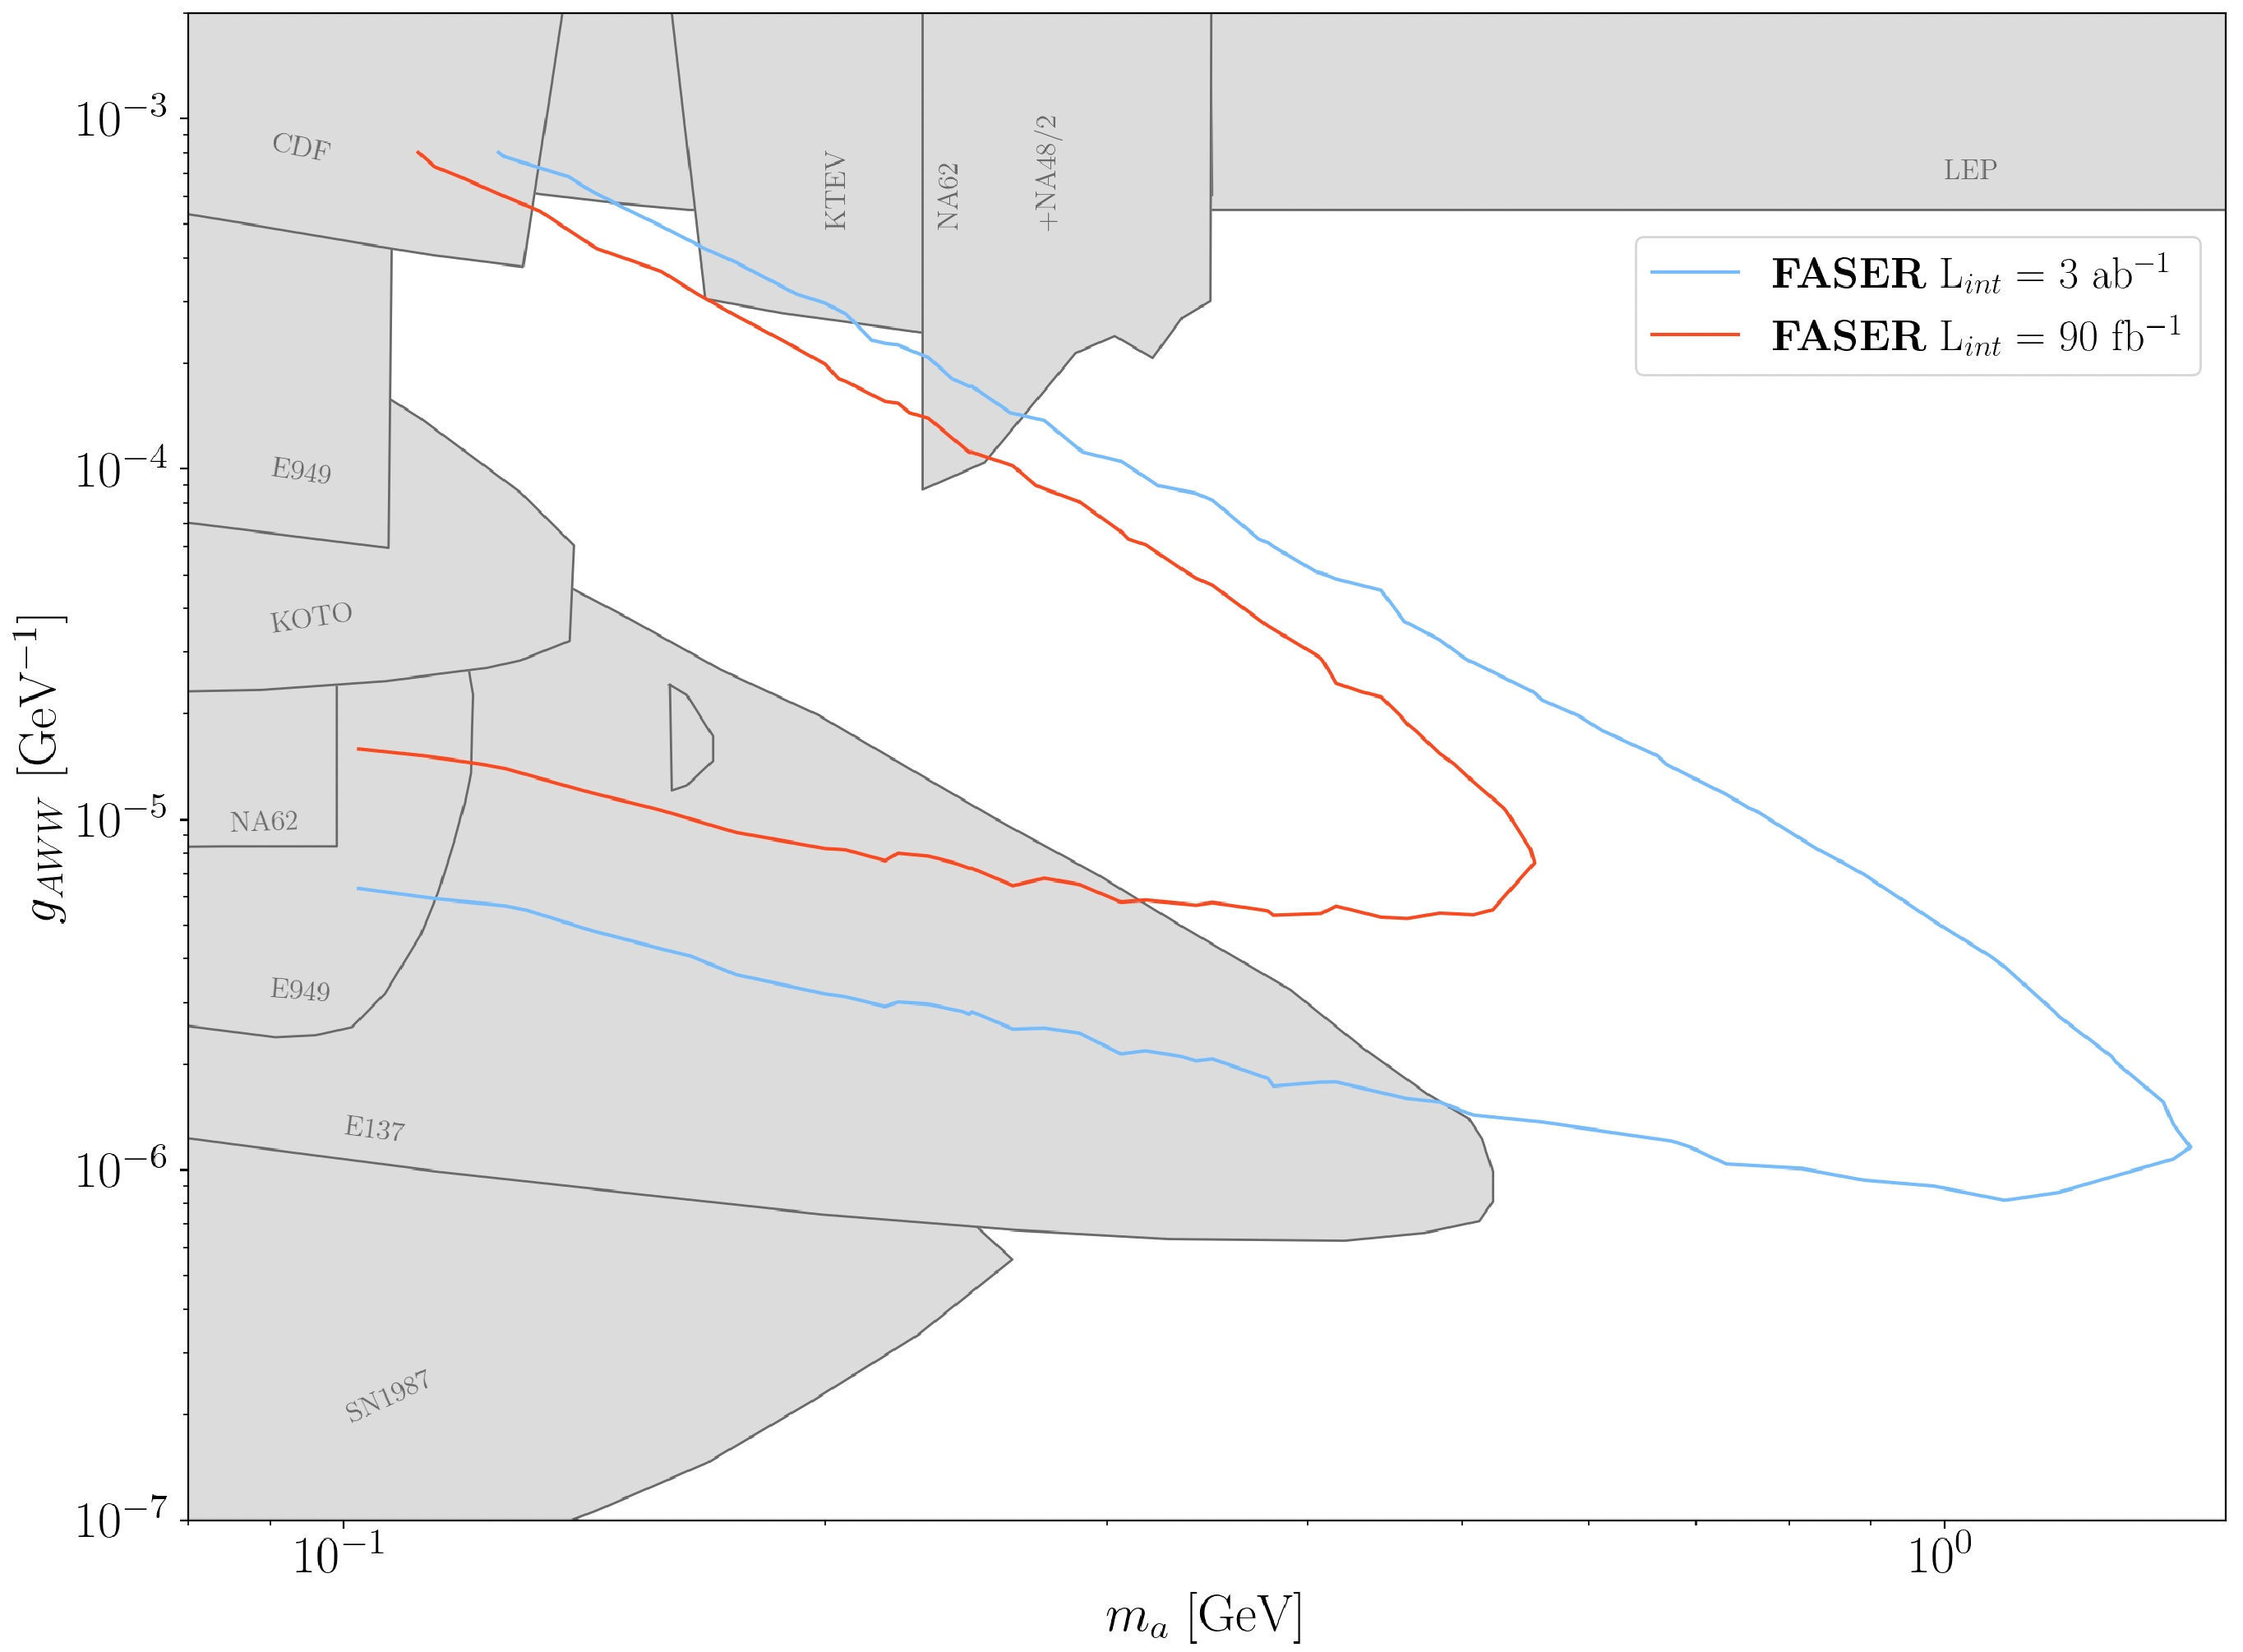
\includegraphics[width=0.8\linewidth]{files/reach_plot_ideal}
			\caption{Sensitivity reach plot for ALP decay into a photo pair wit the FASER detector assuming full detection efficiency. The areas in grey correspond to region in the parameter space already constrained by other experiments. The reach is given for an integrated luminosity of 90 fb$^{-1}$ for the LHC Run 3 (in red) and for 3000 fb$^{-1}$ for the HL-LHC.}
			\label{im:reach_plot_ideal}
		\end{figure}
		
		As one could easily guess, there exists no detection system, even as elegant as one could imagine, that is able to produce a detection efficiency of 100 $\%$. For the sake of having a more truthful description of the discoveries prospects, a detector layout with its main characteristics needs to be specific. This will be the argument addressed in the ensuing discussion. 
		
		\subsection{Sensitivity reach with new PreShower detector}
		
		The detection of the two photons produced in ALPs decay can be performed through the detection of the electromagnetic shower produced by photon converting in an absorber material. Since the produced ALPs are very boosted, the photons will be emitted very close-by and a detector with fine granularity in the transverse plane is required. In order to have redundancy and avoid identifying as photon showers fake events or statistical fluctuation in the shower development, having a sampling over various detector planes of the shower profile can be an advantage. 
		
		In 2020 at the University of Geneva (UniGe), the idea of replacing the original pre-shower station with a fine granularity pre-shower saw light for the first time. In parallel to the studies of ALP production in a novel channel, a first design of the new pre-shower was first drown. The pre-shower's layout remained quite simple and was made of six identical planes composed of roughly 1.3 $X_0$ on tungsten for the absorber part and a plane of monolithic silicon pixel detector for detecting the photon electrons and positrons generated in the electromagnetic shower from the converted photons. It is then interesting to see how the typical decay signatures in FASER would be with the upgraded layout. The signatures are presented in figure \ref{im:FASER_DP_signature_newPS} and figure \ref{im:FASER_ALP_signature_newPS}. 
		
		\begin{figure}[h]
			\centering
			\includegraphics[width=1.0\linewidth]{files/FASER_DP_signature_newPS}
			\caption{Dark photon typical decay signature with new pre-shower station.}
			\label{im:FASER_DP_signature_newPS}
		\end{figure}
		
		\begin{figure}[h]
			\centering
			\includegraphics[width=1.0\linewidth]{files/FASER_ALP_signature_newPS}
			\caption{ALP typical decay signature with new pre-shower station.}
			\label{im:FASER_ALP_signature_newPS}
		\end{figure}
		
		The new typical signatures for the dark photon and ALP decay are to be compared with figure \ref{im:FASER_OLD_DP_signature} and figure \ref{im:FASER_OLD_ALP_signature} respectively. For the dark photon studies, the additional position measurement brought by the six pixel detector planes could help improve the quality of the signal in the case of very close-by tracks. For the ALP, it is possible to distinguish between events with one or more photons as the preshower makes photons converts in the tungsten and the 6 detectors planes are sampling the development of the electromagnetic shower. 
 		  
		In the detector specifications proposed at the time of the studies, the pixel pitch was considered to be \SI{100}{\micro\meter}, meaning that the photons would need to be separated by at least \SI{200}{\micro\meter} to be distinguishable. Simulations of the detector performance with GEANT4 were performed. ALP decay events were produced for two photons whose energies could take any value in $E_\gamma$ = [250, 350, 450, 750, 1000, 1500, 2000, 3500] GeV and for a separations between the photons with values in $\delta_{\gamma\gamma}$ = [0.2, 0.3, 0.5, 1.0, 2.0] mm. An event display of the showers from two photons in the sixth detector plane with energies $E_{\gamma,1} =$ \SI{750}{\giga\electronvolt} and $E_{\gamma,2} =$ \SI{1.5}{\giga\electronvolt} with separation of $\delta_{\gamma\gamma}$ = \SI{200}{\micro\meter} is presented in figure \ref{im:di-photon_event_GEANT4} and was taken from \cite{PreShower_TP}. 
		
		\begin{figure}[h]
			\centering
			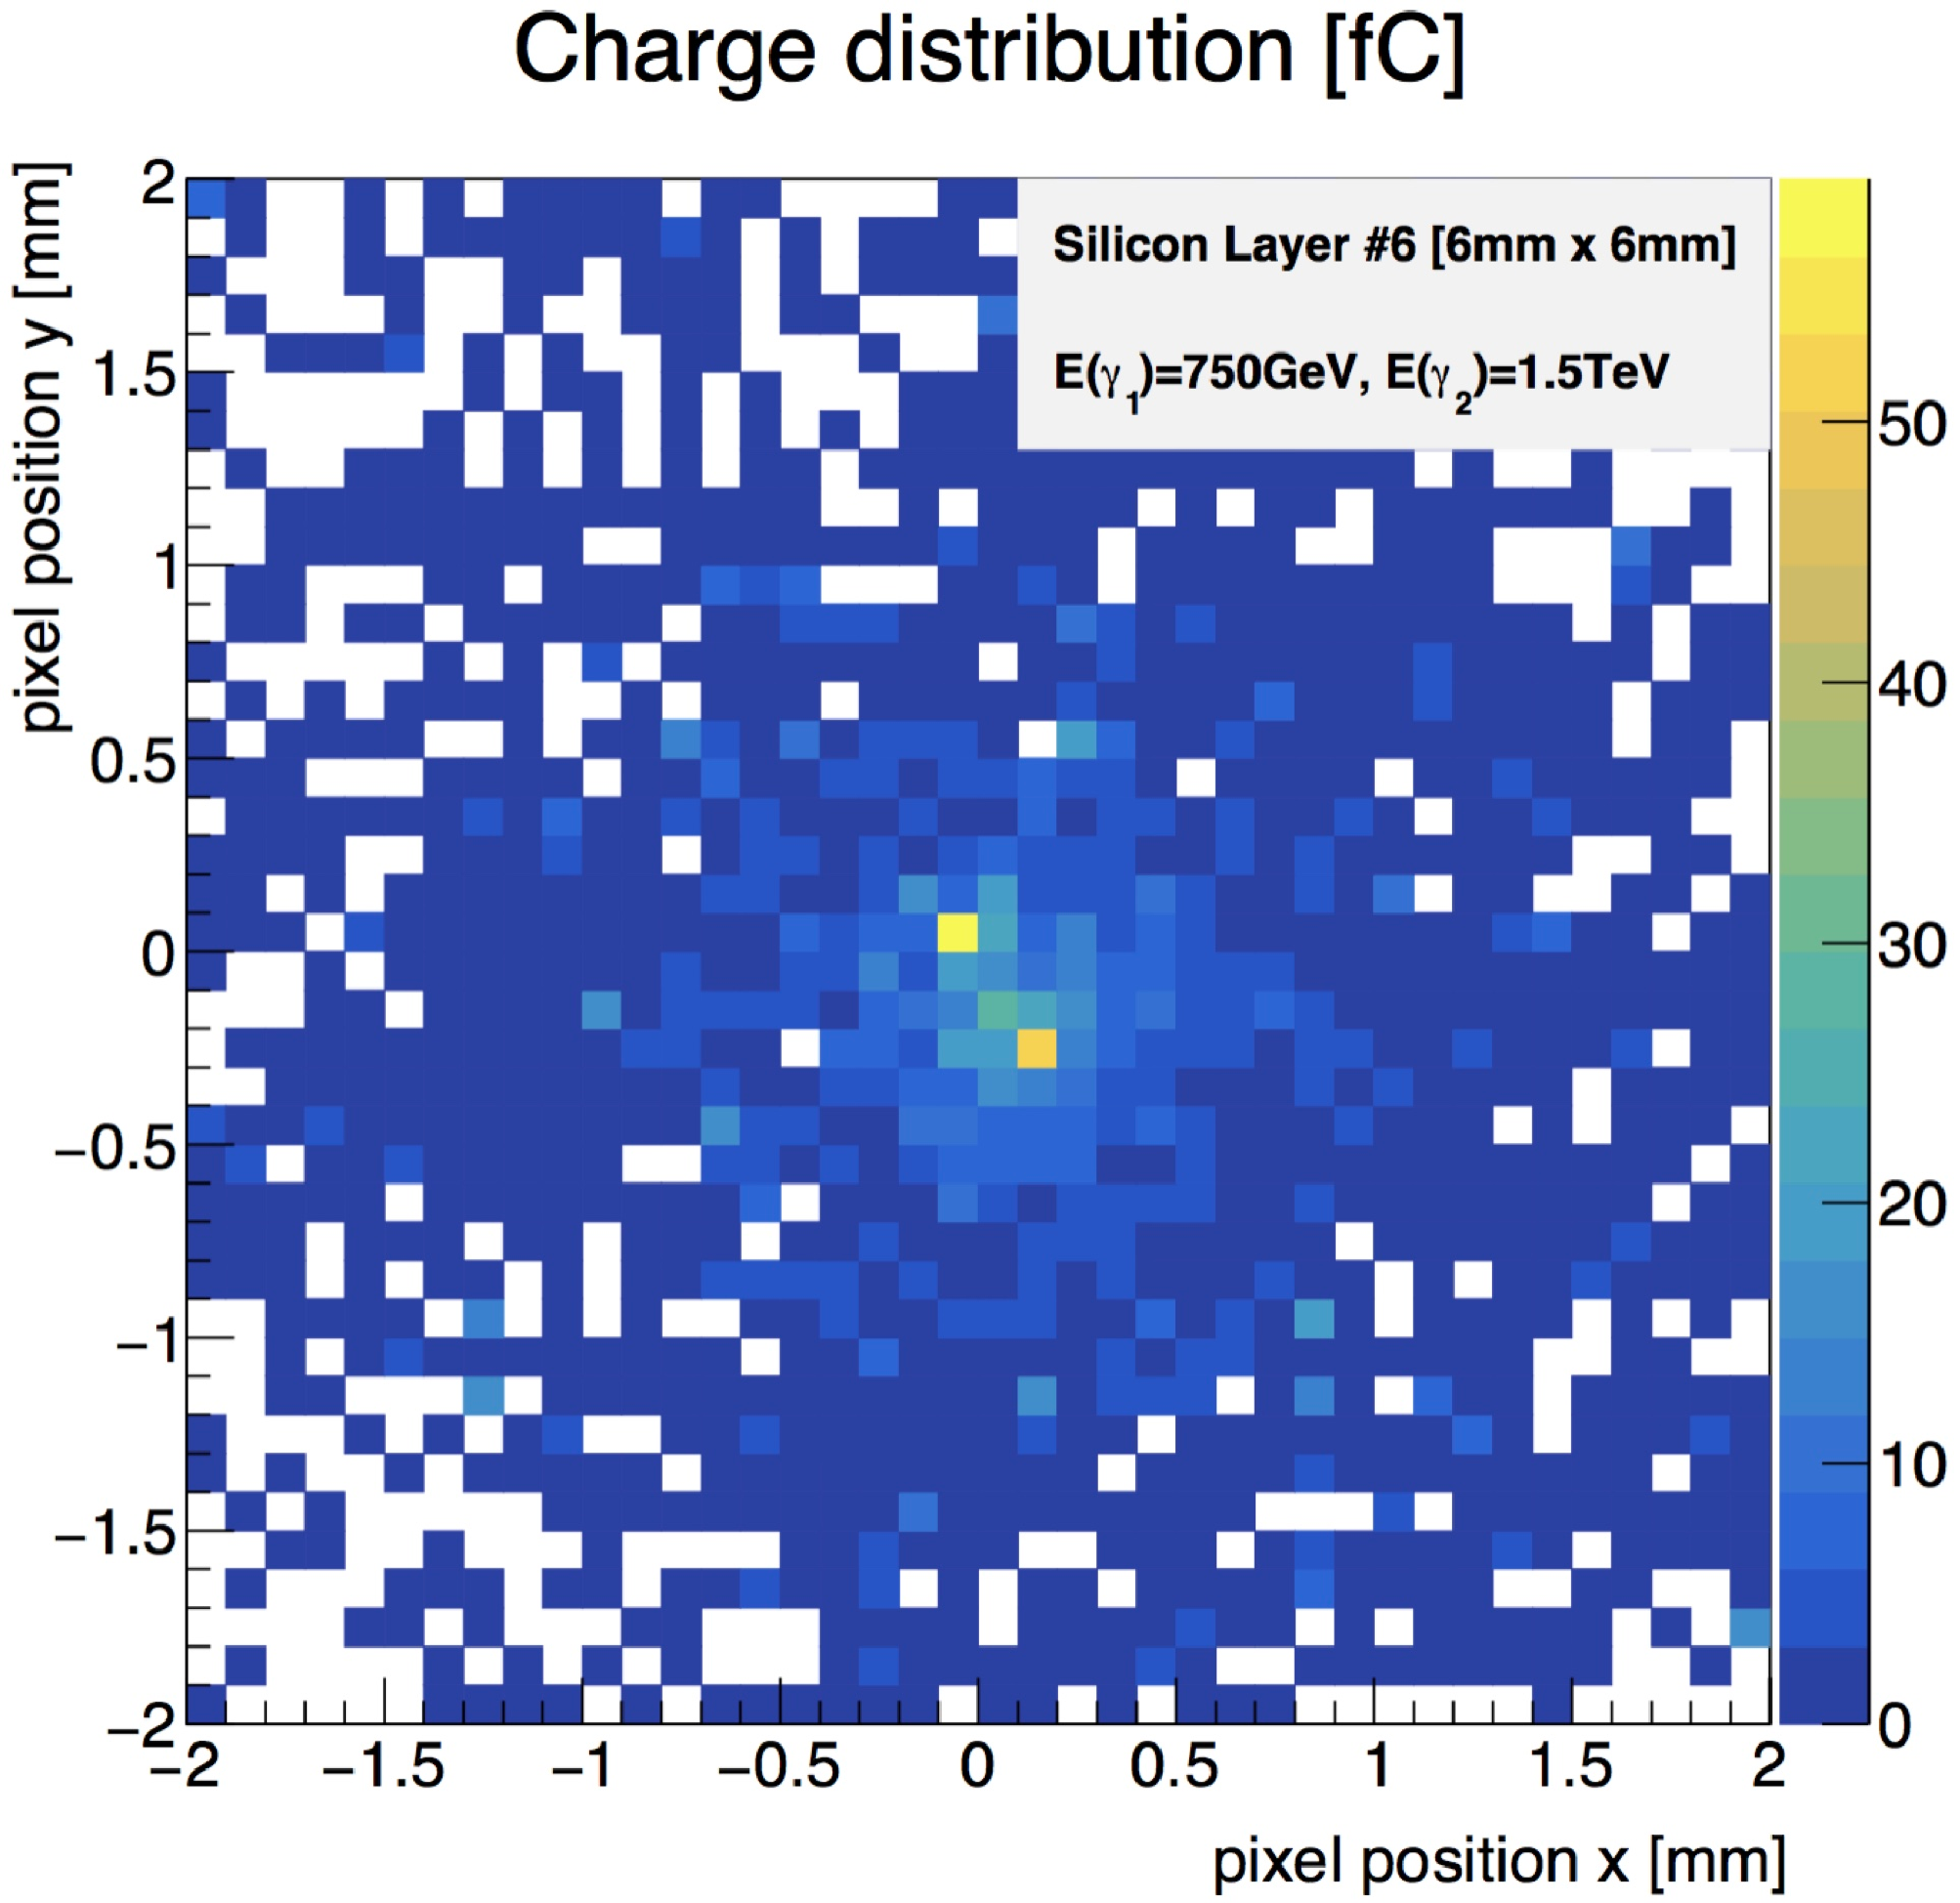
\includegraphics[width=0.7\linewidth]{files/di-photon_event_GEANT4}
			\caption{Event display for the decay of an ALP in two photons with $E_{\gamma,1} =$ \SI{750}{\giga\electronvolt} and $E_{\gamma,2} =$ \SI{1.5}{\giga\electronvolt} and separation $\delta_{\gamma\gamma}$ = \SI{200}{\micro\meter}. The charge deposited by the electromagnetic showers from the two photons is given in fC by the colour scale.}
			\label{im:di-photon_event_GEANT4}
		\end{figure}
		
		The electromagnetic showers from each photon are mixing and are characterised by a low charge deposition across a large region with a much higher charge deposition at the center of the shower fo each individual photon. The position of the photon can be reconstructed as the center of shower where the amount of deposited charge is the highest. A simple photon-reconstruction algorithm was developed to reconstruct the position of the photons using the charge deposition in each pixel across the different detector planes \cite{PreShower_TP}. The detection efficiency was estimated for all of the possible combinations of photon energies and separations cited previously.  
		
		The minimal separation between the photons to be distinguished will have an effect on the number of ALP signals FASER will be able to identify as so. Taking the discussion back into the MC simulations for the ALP, once can see what the effect of the minimal photon separation would be on the distributions previously presented in figure \ref{im:ALP_E1E2_distribution}. The results are presented in figure \ref{im:ALP_E1E2_distribution_cut} and were taken from \cite{Moretti_MasterThesis}. 
		 
		\begin{figure}[h]
			\centering
			
\includegraphics[width=1.0\linewidth]{files/ALP_E1E2_energy_cut}
			\caption{Energy distribution of the photon emerging from ALP decays for different combination of ALP mass $m_a$ and coupling $g_{aWW}$. A selection of events was performed with the criteria that the separation between the two photons when reaching the preshower is greater than $\delta_{\gamma\gamma}$ = \SI{200}{\micro\meter}. The number of events in the top right corner of every figure is given for an integrated luminosity of 90 fb$^{-1}$. The top number is the number of events after the selection criteria while the bottom number is the total number of events.}
			\label{im:ALP_E1E2_distribution_cut}
		\end{figure}
		
		It is striking to observe that a large part of the number of events can disappear, as for example for the benchmark model with mass and coupling values $\left[0.165, 1.8\cdot 10^{-4}\right]$, when comparing figure \ref{im:ALP_E1E2_distribution} and figure \ref{im:ALP_E1E2_distribution_cut}, one can see that the region with photon energy very similar to one another disappeared, leading to a decrease of the number of events of more than 50$\%$. It is also interesting to note that the effect is less important for ALP with lower average energies (as for example the benchmark model with values $\left[0.32, 3.2\cdot 10^{-5}\right]$). Indeed the higher the momentum of the ALP, the more important the Lorentz boost when computing the angles of emission of the photons in the laboratory reference frame and the closer the photons. \\
		
		In order to adapt the sensitivity reach presented in figure \ref{im:reach_plot_ideal} for a more realistic detector, one would need to add the reach as a function of the minimum separation between the photons as it has a drastic effect on the number of events. The number of events was then estimated as a function of the energy of the two photons and their separation for every ALP model with mass $m_a$ and coupling $g_{aWW}$. The number of events where the scaled to the detection efficiencies obtained with the GEANT4 MC simulations and the obtained results from \cite{Moretti_MasterThesis} are shown in figure \ref{im:reach_plot_detector}.
		\begin{figure}[h]
			\centering
			
\includegraphics[width=1.0\linewidth]{files/reach_plot_detector}
			\caption{Sensitivity reach of the new FASER pre-shower detector for different separations between photons. The results are presented for an integrated luminosity of 90 fb$^{-1}$ (left) and 3000 fb$^{-1}$ (right).}
			\label{im:reach_plot_detector}
		\end{figure}
		The results show that the reach for a fixed integrated luminosity changes a a function of the criteria on the minimum separation between the two photons. As expected, the larger the separation criteria and the lower the number of events, this leads to the reach shrinking for higher separations values. Nonetheless, even with a minimal separation of \SI{200}{\micro\meter}, the deviation from the ideal reach is not significant and a large portion of the yet unconstrained parameter space could be probed by FASER. 
		
		In addition to the enhanced sensitivity to ALP di-photon signals, the new design of the pre-shower station will also contribute to the dark photon searches or any model with similar final state ( pair of oppositely charged leptons). The pre-shower allows for more measurements of charged particles at the back of the detector and with a better spatial resolution than the original detector. The addition of this position measurement could allow to separate very closely spaced tracks which can't be separated with the current detector and could even allow for an increase of the length of the decay volume to include the second magnet, increasing the acceptance by 70$\%$ \cite{PreShower_TP}. The pre-shower will also make the overall detector more robust to inefficiencies in the back tracing station. 
		The drawback fo the new pre-shower design is the amount of material present in front of the calorimeter. A degradation in the energy resolution of the calorimeter station could be expected but a correction using the charge measured in the different pre-shower detector planes could help. Nevertheless, it is not expected that the degradation of the energy resolution will have a significant impact on the physics of FASER \cite{PreShower_TP}.\\
		
		The discussion on the FASER detector and its physics program is now over. a few of the leading BSM models in the sensitivity reach of FASER were discussed together with the prospects in reaching higher sensitivity for any model predicting a photonic final state such as the ALP model discussed. The introduction of a "monolithic silicon pixel detector" for the active parts of the new pre-shower station was actually a good hint to the argument discussed in the next chapter. 
		


		
		
		
		
		
		
		
		
		
		
		
		
		
		
		
		
		
		